\chapter{Modèle de coût énergétique pour des requêtes isolées et concurrentes}
\label{chap4}

\epigraph{<< Passion is energy. Feel the power that comes from focusing on what excites you. >>}{--- \textup{Oprah Winfrey}}

\NoChapterPrefix \NoChapterNumberInRef {\hypersetup{linkcolor=black} \minitoc}

%% numérotation des figures, des tables et des équations préfixé par le numéro de chapitre
\makeatletter
\renewcommand{\thefigure}{\ifnum \c@section>\z@ \thechapter.\fi
 \@arabic\c@figure}
\@addtoreset{figure}{chapter}
\makeatother

\makeatletter
\renewcommand{\thetable}{\ifnum \c@section>\z@ \thechapter.\fi
 \@arabic\c@table}
\@addtoreset{table}{chapter}
\makeatother

\makeatletter
\renewcommand{\theequation}{\ifnum \c@section>\z@ \thechapter.\fi
 \@arabic\c@equation}
\@addtoreset{equation}{chapter}
\makeatother
%%-----------------------------------------------------------------
%% Résumé
%%-----------------------------------------------------------------


%laisser une page ou deux pages vides, telle est la question !
%\EmptyNewPage
\newpage

%********************************************************************************
%********************************************************************************
\section{Introduction}
% DONE add glossary for BD, SGBD, 

La consommation d'énergie dans les BD est devenue un vrai problème pour la communauté d'informatique verte ainsi que pour les scientifiques et les administrateurs de BD. L'énergie doit être optimisée à plusieurs niveaux : matériel, système d'exploitation et SGBD. Toutefois, l'estimation du coût énergétique dans les opérations de BD a une importance majeure dans la conception de BD minimisant l'énergie. En effet, c'est la première étape à réaliser dans la plupart des techniques d'optimisation logicielles. Les solutions existantes (voir \ref{chap3}) proposent des approches limitées pour la mesure de l'énergie d'une manière efficace et précise. Celles-ci s'avèrent simples, ne considérant pas les requêtes complexes, ou ne sont pas portables dans différentes configurations n'ayant pas de modèle mathématiques robuste.

Nous présentons dans ce chapitre le modèle de coût que nous avons proposé pour estimer l'énergie consommée par une requête donnée. Nous commençons par présenter les motivations d'utilisation d'un modèle de coût énergétique dans notre approche. Nous présentons ensuite les hypothèses que nous avons considérées pour établir ce modèle de coût. Nous donnons la démarche de construction de notre modèle, à savoir l'identification des paramètres, le niveau de modélisation et la technique de régression. Nous proposons deux types de modèles de coûts : (1) un modèle de coût pour les requêtes exécutées d'une manière isolée et (2) un pour le cas des requêtes concurrentes ou parallélisées. Enfin, nous évaluons notre modèle contre des benchmarks réels avec différentes configurations physiques pour montrer l'utilité et l'efficacité de notre approche.

\section{Pourquoi un modèle de coût ?}\label{sec:PourquoiModelCout}

Les modèles de consommation d'énergie sont très importants pour de nombreux systèmes où l'on exige une efficacité énergétique \cite{Rivoire08phd}. La conception du matériel informatique utilisé par les centres de données nécessite un modèle de coût, car il est impossible de construire des systèmes physiques afin d'évaluer tous les effets des choix de conception sur la consommation d'énergie. Dans l'utilisation quotidienne des systèmes informatiques, les utilisateurs et les opérateurs de centres de données doivent savoir et comprendre comment leurs modes d'utilisation affectent la consommation d'énergie de la machine afin de maximiser son efficacité énergétique, que ce soit dans un seul système ou sur un ensemble de systèmes. L'utilisation d'un matériel de mesure n'est pas une solution, car il ne peut pas prédire l'énergie, et il est généralement coûteux et inflexible face au changement des systèmes. Finalement, les modèles de coût permettent de développer des techniques d'optimisation de la consommation d'énergie.

Une modélisation d'énergie idéale adaptée à une utilisation dans les BD devrait répondre à plusieurs critères de conception. La modélisation basée seulement sur le matériel ne peut pas répondre à ces critères, car elle ne peut pas prédire la consommation d'énergie des futures requêtes, et elle ne décrit pas le lien entre l'utilisation des ressources et la consommation d'énergie, qui est nécessaire pour l'optimisation d'efficacité énergétique des BD. Les principaux critères sont :

\begin{itemize}
 \item \textbf{La précision.} Le modèle doit être suffisamment précis lors des estimations d'énergie. Une erreur importante dans les résultats risque de générer de mauvaises décisions lors de la phase d'utilisation du modèle.
 \item \textbf{La portabilité et la robustesse.} Le modèle doit maintenir une grande précision indépendamment des variations des systèmes matériels ou logiciels, et les caractéristiques de la charge de requête. La génération du modèle pour un nouveau système doit être facile et ne requiert pas une re-conception.
 \item \textbf{La rapidité.} Le modèle doit générer des prédictions assez rapidement pour être exploitées dans les optimisations en temps réel.
 \item \textbf{La simplicité.} Le modèle doit être simple en terme de nombre de paramètres d'entrée et en complexité algorithmique. Il ne doit pas impliquer des paramètres autres que ceux utilisés par les SGBD traditionnels. 
 \item \textbf{La faible surcharge.} Le processus de modélisation ne doit ni interférer avec les activités normales du SGBD, ni impliquer des modifications importantes sur le matériel. Il ne devrait pas générer une surcharge du système.
 %DONE modifications importantes sur le matériel?? je dirai faire de multiples appels au matériel?
\end{itemize}

\subsection{Approches de modélisation}
Dans la littérature, il existe deux approches pour modéliser l'énergie d'un système : (1) une approche \textit{analytique} (boite blanche) ou (2) une approche \textit{expérimentale} (boite noire) \cite{Rivoire08}. Chaque approche a ses avantages et ses inconvénients. L'approche analytique modélise un système dont on peut prévoir le fonctionnement interne car on connaît les caractéristiques de fonctionnement de l'ensemble des éléments qui le composent. La connaissance détaillée des éléments du système rend le modèle plus précis. Par contre, cette approche est complexe à réaliser, puisqu'elle implique un grand nombre de paramètres et requiert un temps de calcul important et une grande capacité de calcul et de maintenance face à l'évolution du système.

Une approche expérimentale fournit quant à elle la représentation d'un système sans considérer ni son fonctionnement interne, ni son architecture. Elle se base seulement sur les données des expérimentations et les techniques d'identification. La mise en œuvre de ce types d'approches est simple et rapide puisqu'elle ne requiert pas une connaissance approfondie du système. En revanche, la non-connaissance des composantes du système et leur comportement influence sur la qualité des résultats du modèle final. Le modèle peut avoir besoin d'une nouvelle adaptation si le système change.

Nous proposons de combiner les deux approches afin de profiter des avantages de chacune, en traitant le système comme une \textit{boite grise}. Cette approche prend en compte une partie du fonctionnement interne du système d'un côté et se base sur des données expérimentales de l'autre côté. Dans la pratique, nous allons lancer des expérimentations pour mesurer l'énergie du système et étudier sa variation suivant les caractéristiques de la charge de requêtes, afin de trouver les paramètres et les fonctions mathématiques clés qui décrivent la consommation d'énergie du système. La \ref{fig:modelling-approaches} résume les trois approches de modélisation citées ci-dessus.

\begin{figure}
 \centering
 \includegraphics[scale=0.60]{chapitre4/chap4Fig/modelling-approaches.pdf}
 \caption{Les approches de modélisation d'énergie.}
 \label{fig:modelling-approaches}
\end{figure}

\subsection{Niveau de modélisation}
Lorsqu'une requête SQL est soumise à un SGBD, elle sera traduite en un arbre d'opérateurs algébriques puis en plan d'exécution. L'optimiseur de requêtes applique des fonctions analytiques pour trouver le meilleur plan d'exécution. Ensuite, la requête sera exécutée suivant un mode itératif (pipeline), où un ensemble d'opérateurs algébriques s'exécutent en même temps lorsqu'il y a des données à traiter.
Intuitivement, la modélisation d'énergie d'une requête,  peut se faire à trois niveaux :

\begin{enumerate}
 \item \textbf{Niveau requête.} Considérer les caractéristiques de la requête elle-même, telles que le nombre d'entrées/sorties requises pour exécuter la requête. Ce niveau est facile à mettre en œuvre mais ne garantis pas la précision désirée.
 \item \textbf{Niveau pipeline.} Considérer les caractéristiques de l'ensemble d'opérateurs qui s'exécutent simultanément. Le défi dans ce niveau est la détermination de ces opérateurs.
 \item \textbf{Niveau opérateur.} Considérer les caractéristiques de l'opérateur individuellement. La modélisation à ce niveau exige des détails sur les opérateurs et leurs implémentations, ce qui rend le processus complexe.
\end{enumerate}

Le bon choix du niveau de modélisation est crucial pour la qualité du modèle final. Ce choix peut se faire à l'aide d'une étude expérimentale comme décrit dans la section précédente. %DONE no comprendo la derniere phrase

\subsection{Mode d'exécution des requêtes}
La plupart des SGBDs modernes sont des systèmes multi-utilisateurs où plusieurs utilisateurs peuvent se connecter à la BD et exécuter des requêtes de façon concurrente. Il incombe au SGBD de gérer la concurrence d'accès aux données, et de garantir la fiabilité des résultats des requêtes. Comme nous allons montrer, la consommation énergétique pour une seule requête n'est pas forcément la même pour un ensemble de requêtes qui s'exécutent en même temps en parallèle. Par conséquent, il existe deux modes d'exécution de requêtes à considérer dans la phase de conception d'un modèle de coût énergétique : (1) le mode isolé et (2) le mode concurrent.

\begin{enumerate}
 \item \textbf{Mode isolé.} Une seule requête est en train d'être exécutée de façon isolée par le SGBD dans une instance donnée. Ce mode est la base de toute conception d'un modèle de coût énergétique due à sa complexité réduite.
 \item \textbf{Mode concurrent.} Plusieurs requêtes sont en train d'être exécutées de façon concurrentes par le SGBD dans une instance donnée. Ce mode est plus générique que le premier et plus utile pour de nombreuses tâches de gestion de BD, à l'exemple du contrôle d'admission, l'ordonnancement des requêtes et de contrôle d'exécution. Cependant, la conception de ce mode est plus complexe.
\end{enumerate}

\section{Démarche pour la construction d'un modèle de coût énergétique}\label{DemarcheConstruction}
Dans cette section, nous présentons notre méthodologie pour créer un modèle de coût qui estime la consommation d'énergie d'une seule requête SQL.
Nous adoptons une approche logicielle basée sur une étude empirique pour trouver les paramètres clés ayant un impact sur l'énergie, et pour identifier le niveau adéquat pour modéliser l'énergie des requêtes. L'étude empirique permet aussi de sélectionner l'algorithme mathématique qui modélise mieux le comportement de l'énergie des requêtes SQL. Les principales étapes pour développer notre modèle de coût sont (cf. \ref{fig:costmodel-methodology}) :

\begin{itemize}
 \item \textbf{Identification des paramètres.} Afin de réduire la consommation d'énergie d'un système, nous devons d'abord mesurer la consommation d'énergie de ses composantes et identifier là où la plupart de l'énergie est dépensée. Ceci est la tâche de la phase d'extraction des paramètres du modèle. Elle prend comme entrée le matériel utilisé, le SGBD et la charge de requêtes.
 \item \textbf{Construction du modèle.} Les paramètres d'entrée sélectionnés précédemment sont utilisés pour construire le modèle de consommation d'énergie en utilisant des techniques \textit{analytiques} ou \textit{statistiques} telles que la régression, l'apprentissage automatique, etc. L'un des principales difficultés de cette étape est que certains paramètres importants du système tels que la consommation d'énergie d'un composant particulier, ne peuvent pas être mesurés directement. Les méthodes analytiques classiques peuvent ne pas produire des résultats précis dans de telles situations, les techniques d'apprentissage automatique peuvent donner de meilleurs résultats.
 \item \textbf{Validation et utilisation.} Le modèle doit être validé selon différents scénarios pour son adaptation à ses fins prévues. Il peut être utilisé a postériori comme une base pour prédire la consommation d'énergie des requêtes. Ces estimations peuvent ensuite être utilisées pour améliorer l'efficacité énergétique des SGBD, par exemple en incorporant le modèle dans des techniques d'optimisation telles que la conception physique, l'ordonnancement des requêtes, l'ajustement dynamique de la fréquence de la tension (DVFS), l'amélioration des algorithmes et ainsi de suite.
\end{itemize}

\begin{figure}
 \centering
 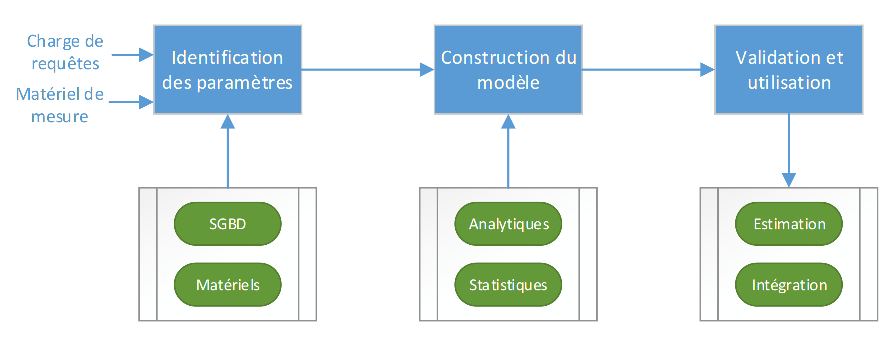
\includegraphics[scale=0.8]{chapitre4/chap4Fig/costmodel-methodology.eps}
 \caption{Les étapes de développement de notre modèle de coût énergétique.}
 \label{fig:costmodel-methodology}
\end{figure}

\subsection{Nos hypothèses}
% DONE Stéphane "le méticuleux" m'a déconseillé l'utilisation des abrévéations p. ex./c-a-d .. a toi de voir
Dans notre étude, et à cause de la complexité du problème traité, nous limitons les possibilités liées à l'environnement. La multitude des environnements (p. ex. centralisé, distribué et parallèle), des SGBD (p. ex. relationnel, NoSQL ou NewSQL) ou encore des requêtes (p. ex. sélection et mise à jour) rend la démarche plus complexe. Dans notre travail, nous considérons les hypothèses suivantes :
%DONE remplir les points de suspension. A moin avis ne pas justifier car c'est evident, dire simplement, Nous présentons, ci-dessous, les hypothèses que nous avons considérées pour établir ces MdC.
\begin{enumerate}
 \item L'environnement de travail est centralisé, la BD est déployée dans une seule station de travail. Par conséquent, le coût de communication est ignoré.
 \item Nous ne considérons pas des requêtes de définition de données (p. ex. \texttt{CREATE}, \texttt{DROP}, \texttt{ALTER}) ou encore de requêtes de manipulation de données (p. ex. \texttt{INSERT}, \texttt{DELETE}, \texttt{UPDATE}). Les requêtes considérées sont de type transactionnel et analytique, ayant la forme suivante :
 %\begin{lstlisting}[caption=An OCL structural rule, label=lst:listingocl]
 \begin{lstlisting}[language=Sql]
SELECT [DISTINCT ou ALL] colonnes
FROM tables
[WHERE predicats]
[GROUP BY expression]
[HAVING condition]
[ORDER BY colonnes]
\end{lstlisting}
 \item Les requêtes sont exécutées de façon isolée et concurrente (c-à-d parallélisme inter-requêtes).
 \item Le cache est vidé entre l'exécution des requêtes.
\end{enumerate}

\subsection{Identification des paramètres}
La première étape de notre approche est l'identification des paramètres clés de notre modèle qui influencent sur la consommation d'énergie des requêtes. L'identification est réalisée suivant une approche d'apprentissage automatique. Cette stratégie expérimentale est utilisée lorsque les paramètres du $\mathcal{BNF}$ sont inconnus au préalable. Dans cette stratégie, nous testons l'exécution de plusieurs requêtes simples et complexes, isolées et concurrentes, dans différentes BD et de tailles différentes, puis nous observons les paramètres liés à la stratégie d'exécution des requêtes, les caractéristiques de la BD et le matériel utilisé.

\subsubsection{Effet de stratégie d'exécution des requêtes}
Pour étudier l'effet de la stratégie d'exécution des requêtes sur la consommation d'énergie, nous commençons par montrer un exemple de la requête \textit{Q9} du benchmark TPC-H \cite{TPCH}. La \ref{fig:tpch-q9-sql} montre la syntaxe de cette requête qui détermine le bénéfice de la vente d'une ligne de pièces, groupé par la nation et l'année des fournisseurs.

Les ensembles de données et la configuration du système que nous avons utilisés dans nos expérimentations peuvent être trouvés dans la \ref{sec:experiment}.
La \ref{fig:tpch10-set1-q9-power} montre la consommation d'énergie active pendant l'exécution de la requête qui a débuté à la 10\textsuperscript{ème} seconde et a fini à la 143{ème} seconde. Nous pouvons y distinguer trois segments différents qui s'avèrent correspondre à la segmentation en \textit{pipelines}. Ces derniers permettent l'exécution simultanée d'une séquence contiguë d'opérateurs SQL souvent implémentés selon un modèle itératif \cite{Connolly05}.

La segmentation en pipelines du plan d'exécution de la requête \textit{Q9} est montrée dans la \ref{fig:tpch10-set1-q9-tree}. Il y a 7 pipelines dont l'ordre d'exécution est déterminé par leurs opérateurs \textit{bloquant} (p. ex. $PL6$ ne peut pas commencer avant que $PL5$ soit terminé). Bien que la requête a sept pipelines différents, seulement quatre sont importants dans notre discussion (les autres terminent très rapidement).
La détermination des segments énergie-pipelines est effectuée à l'aide du \textit{module de surveillance SQL temps réel} intégré dans le SGBD \cite{Sergey09}, qui nous donne en temps réel les statistiques à chaque étape du plan d'exécution avec le temps écoulé. Sur la base de ces informations, nous avons segmenté l'intervalle de l'énergie en pipelines correspondants.

\begin{figure}
\begin{lstlisting}[language=sql]
select nation, o_year, sum(amount) as sum_profit
from
	(
		select
			n_name as nation, extract(year from o_orderdate) as o_year,
			l_extendedprice * (1 - l_discount) - ps_supplycost * l_quantity as amount
		from
			part, supplier, lineitem,
			partsupp, orders, nation
		where
			s_suppkey = l_suppkey and ps_suppkey = l_suppkey
			and ps_partkey = l_partkey and p_partkey = l_partkey
			and o_orderkey = l_orderkey and s_nationkey = n_nationkey
			and p_name like '%sandy%'
	) as profit
group by nation, o_year
order by nation, o_year desc;
\end{lstlisting}
  \caption{La requête \textit{Q9} issue du benchmark TPC-H.}\label{fig:tpch-q9-sql}
\end{figure}

Si l'on compare les intervalles de changement de la consommation d'énergie avec le changement des pipelines dans la \ref{fig:tpch10-set1-q9}, nous pouvons voir que \textit{lorsqu'une requête passe d'un pipeline à l'autre, sa consommation d'énergie également change}. Au cours de l'exécution d'un pipeline, la consommation d'énergie a généralement tendance à être stable.
L'hypothèse faite par Xu \textit{et al.} stipulant que lors de l'exécution d'une seule requête dans un système, le coût de l'énergie est stable (steady state) \cite{Xu12} s'avère donc être fausse. En effet, de nombreuses requêtes ont différents segments de consommation d'énergie au cours de leur exécution. Ceci est dû au fait que l'estimation de Xu \textit{et al.} a été réalisée au niveau de la requête. Pour avoir des modèles de coûts d'énergie plus précis, l'estimation doit être effectuée au niveau plus fin qui constitue les pipelines.

\begin{figure}[!ht]
  \centering
  \subfloat[La segmentation de la consommation d'énergie suivant les pipelines\label{fig:tpch10-set1-q9-power}]{
    \centering
    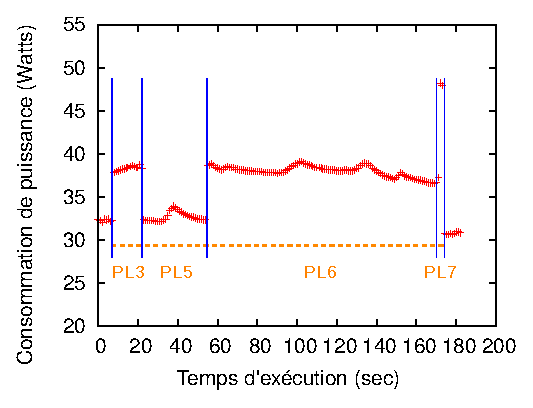
\includegraphics[width=0.5\textwidth]{chapitre4/chap4Fig/tpch10-set1-q9-5.eps}
  }
  \quad
  \subfloat[La segmentation du plan d'exécution suivant les pipelines\label{fig:tpch10-set1-q9-tree}]{
    \centering
    \includegraphics[width=0.4\textwidth]{chapitre4/chap4Fig/tpch-10go-q9-plan.pdf}
  }
  \caption{La consommation d'énergie et le plan d'exécution de la requête \textit{Q9} issue du benchmark TPC-H avec l'annotation des pipelines correspondante.}\label{fig:tpch10-set1-q9}
\end{figure}

\subsubsection{Effet de la taille de BD}
Habituellement, nous admettons le fait suivant : \textit{<< grande taille, plus d'énergie >>}. Pour vérifier ce fait, nous menons des expérimentations, en termes de consommation de puissance active, en tenant compte des requêtes du benchmark TPC-DS \cite{TPCDS} avec deux ensembles de données. Le premier ensemble est de taille 10 Go et le second de 100 Go.
Nous voyons clairement dans le \ref{tab:query-comp}, que les requêtes interrogeant une petite taille de données peuvent  \textit{parfois} consommer plus de puissance que des requêtes interrogeant une grande taille de données. Nous avons créé un autre jeu de données du benchmark TPC-H avec des requêtes modifiées et nous avons trouvé le même comportement (les résultats ne sont pas présentés car ils sont très semblables). Nous notons ici que le plan d'exécution généré par le SGBD pour chaque requête est le même dans les deux ensembles de données.

\begin{table}[]
\centering
\caption {Comparaison de la consommation de puissance active des requêtes du benchmark TPC-DS avec différentes tailles de BD.} \label{tab:query-comp}
%\rowcolors{0}{}{lightgray}
\begin{tabular}{ccc}
%\begin{tabular}{@{}ccc@{}}
\toprule
\multirow{2}{*}{\textbf{Requête}} & \multicolumn{2}{c}{\textbf{Puissance d'électricité (W)}} \\ \cmidrule(l){2-3} 
                                & \textbf{10 Go}                  & \textbf{100 Go}                 \\ \midrule
	$Q4$           & 44,6       & 40,6        \\ 
    $Q9$           & 42,7       & 37,4        \\ 
    $Q11$          & 43,9       & 40,9        \\ 
    $Q39$          & 42,9       & 38,5        \\ 
    $Q48$          & 47,0       & 37,9        \\     
    $Q72$          & 36,4       & 34,1        \\ 
    $Q88$          & 43,3       & 37,6        \\ \bottomrule
\end{tabular}
\end{table}

Nous expliquons ce constat par le fait que pour certaines requêtes, la lecture de gros fichiers de données a besoin de plus de tâches d'E/S. Ainsi, lorsque les résultats intermédiaires ne peuvent pas être stockés dans la mémoire, ils seront écrits sur le disque et lus plus tard. Cette manœuvre se traduit par plus de temps d'attente de CPU, car la requête passe son temps dans la lecture/écriture de ses données plus que dans le traitement de ses tuples. Ainsi, les requêtes dominées par des coûts d'E/S ont moins de consommation d'énergie. De l'autre côté, lorsque les données sont de petite taille, la lecture de données termine rapidement et dans son temps restant, l'exécution de la requête est dominée par le traitement du processeur, ce qui peut se traduire par une forte consommation d'énergie.

Cette observation nie la prémisse faite par Xu \textit{et al.} stipulant que la consommation d'énergie marginale (énergie active) d'une requête est positivement liée à la taille de données interrogées \cite{Xu13}. En effet, nous avons trouvé beaucoup de contre-exemples où des requêtes ont une consommation différente indépendamment de la taille de données, comme indiqué précédemment dans le \ref{tab:query-comp}.

Le coût du CPU et le coût des E/S fournis par le SGBD sont candidats pour être les paramètres du modèle pour les raisons suivantes :
\begin{itemize}
 \item ils sont déjà calculés et disponibles à partir du SGBD optimiseur,
 \item ils couvrent un large éventail d'opérateurs SQL mises en œuvre par les SGBD.
\end{itemize}
Nous avons décidé d'utiliser les coûts CPU et E/S en tant que paramètres dans notre modèle, contrairement à Kunjir \textit{et al.} \cite{Kunjir12} qui utilisent le débit et la taille de données comme paramètres pour modéliser la consommation de puissance maximale (peak power).%DONE compléter la ref

\subsubsection{Effet du mode d'exécution des requêtes}
Nous étudions l'effet du mode d'exécution des requêtes (isolé ou concurrent) sur la consommation d'énergie du système. Pour cela, nous utilisons les données et les charges de requêtes issues du benchmark TPC-H. Nous avons créé de nouvelles charges de requêtes pour chaque mode d'exécution à partir des 22 requêtes d'origine en se basant sur un taux de multiprogrammation donné. 
%DONE vérifier cette derniere phrase

\begin{definition}
Un taux de multiprogrammation (\gls{MPL}) est défini comme le nombre de requêtes exécutées en même temps à un instant donné.
\end{definition}
La charge de requêtes contient les mêmes requêtes, mais avec différentes instances. Nous avons exécuté les charges de requêtes et enregistré leurs consommation d'énergie. Ensuite, nous avons calculé la puissance minimale, maximale et moyenne pour chaque MPL. Les résultats sont présentés dans la \ref{fig:mpls-power}. Nous notons que le taux de multiprogrammation \textit{x} signifie que \textit{x} requêtes s'exécutent simultanément.

\begin{figure}
 \centering
 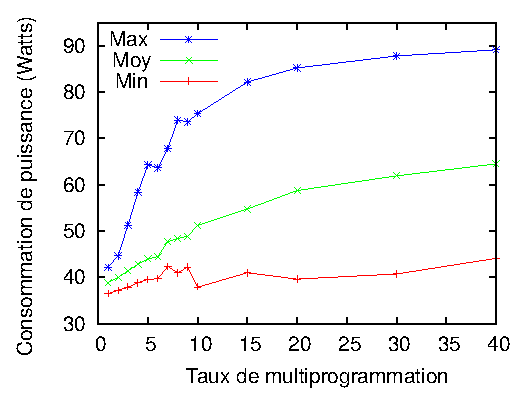
\includegraphics[scale=0.9]{chapitre4/chap4Fig/mpls-power.eps}
 \caption{Variation de la consommation d'énergie de la charge de requêtes suivant les différents taux de multiprogrammation (MPLs).}
 \label{fig:mpls-power}
\end{figure}

Comme prévu, la consommation d'énergie augmente à mesure que l'on augmente le degré de concurrence, car le système devient plus chargé. En fait, le système atteint son débit maximal à \textit{MPL = 40} et consomme sa puissance maximale (95 Watts) tel que mentionné par le fabriquant du matériel. De plus, on observe une grande différence entre le minimum, le maximum, et la moyenne de consommation d'énergie du même MPL. Ainsi, la modélisation pour des requêtes s'exécutant en mode concurrent est largement plus difficile que pour une seule requête autonome. Par conséquent, la considération du mode d'exécution dans la modélisation est cruciale pour une prédiction avec précision de la puissance d'une charge de requête.

Inspiré par les constats des sections précédentes, nous avons conçu et mis en œuvre un modèle d'énergie à base de coût. %L'idée de base de ce modèle est de
La \ref{fig:power-model-building} montre le flux de travaux de notre processus de modélisation d'énergie.
Les caractéristiques de notre modèle comprennent : (1) la segmentation d'un plan d'exécution en un ensemble de segments d'énergie/pipelines suivant les opérateurs bloquants et semi-bloquants, (2) l'utilisation du coût CPU et E/S des pipelines et de l'énergie mesurée on mode \textit{hors ligne} pour construire le modèle et (3) l'estimation de l'énergie des futures requêtes en mode \textit{en ligne} basée sur le modèle de coût final. Ainsi, nous bénéficions des avantages suivants :
\begin{itemize}
 \item nous ne nous appuyons pas sur type d'opérateur SQL ou sur son implémentation physique, car la modélisation de chaque opérateur algébrique est complexe et diffère d'un SGBD à un autre.
 \item notre modèle peut être facilement intégré dans l'optimiseur des SGBD existants.
\end{itemize}

\begin{figure}
 \centering
 \includegraphics[scale=0.55]{chapitre4/chap4Fig/power-model-building.pdf}
 \caption{Le processus de conception du modèle de coût énergétique.}
 \label{fig:power-model-building}
\end{figure}

Dans les sections suivantes, nous détaillons chaque étape de notre processus de modélisation.

\subsection{Segmentation en pipelines}
La deuxième étape de notre approche est la segmentation en pipelines. Quand une requête est soumise à un SGBD, l'optimiseur de requêtes choisit un plan d'exécution. Un plan est un arbre composé d'un ensemble d'opérateurs physiques, tel que la lecture, la jointure ou le tri. La \ref{fig:tpch10-set1-q9-tree} présente un exemple de plan d'exécution renvoyée par l'optimiseur de requêtes. Un opérateur physique peut être \textit{bloquant} ou \textit{non bloquant}.
\begin{definition}
Un opérateur est bloquant s'il ne peut produire aucun tuple sans lire au moins une de ses entrées (p. ex. l'opérateur de tri).
\end{definition}
Basé sur la notion des opérateurs bloquant/non bloquant, nous décomposons le plan d'exécution en un ensemble de pipelines délimités par les opérateurs bloquants. Ainsi, un pipeline est défini comme suit.
\begin{definition}
Un pipeline est un ensemble d'opérateurs s'exécutant simultanément \cite{li12}.
\end{definition}
Comme dans les travaux précédents \cite{chaudhuri04, luo04}, les pipelines sont créés de manière inductive, à partir des opérateurs feuilles du plan à l'instar de l'accès séquentiel et l'accès par index. Chaque fois que nous rencontrons un opérateur bloquant, comme le tri et le groupage, le pipeline en cours se termine et un nouveau commence. Pour une jointure de hachage, l'opérateur de jointure est inclus dans le pipeline du nœud de calcul de jointure (\textit{probe phase} en anglais), et le nœud de la construction de la table de hachage (\textit{build phase}) est la racine d'un autre pipeline. Pour une opération de jointure par tri-fusion, les pipelines contenant ses nœuds d'entrée et l'opérateur de jointure sont réunis pour créer un seul pipeline. Pour une jointure par boucles imbriquées ou boucles imbriquées avec index, les nœuds externes, l'opérateur de jointure et toute sa sous-arborescence des nœuds intérieurs font partie d'un même pipeline.
La définition donnée ci-dessus peut être étendue à d'autres opérateurs physiques. L'\ref{algo:pl-segmentation-algo} illustre un pseudo code de ce principe avec quelques opérateurs, une implémentation en C++ est mentionnée dans le \ref{chap5}. 
Par conséquence, le plan d'exécution d'origine peut être considéré comme un arbre de pipelines. La \ref{fig:tpch10-set1-q9-tree} montre le plan d'une requête ayant 7 pipelines :
\begin{enumerate}
 \item Les pipelines $PL1$, $PL2$, $PL3$, $PL4$ font la lecture séquentielle des tables de données et construisent leur table de hachage en même temps. Ce sont des opérateurs bloquants.
 \item Le pipeline $PL5$ fait la jointure par hachage (opérateurs non-bloquant) entre la table \texttt{LINEITEM} et le $PL1$ puis le résultat avec les autres pipelines. À la fin, le pipeline construit la table de hachage du résultat final.
 \item Le pipeline $PL6$ fait la jointure par hachage entre $PL5$ et la table \texttt{ORDERS} puis le résultat avec le $PL1$.
 \item Le pipeline $PL7$ calcule l'opérateur bloquant qui est le tri de $PL6$ et affiche le résultat final de la requête.
\end{enumerate}

\begin{algorithm}
\caption{Algorithme de segmentation des pipelines}
\label{algo:pl-segmentation-algo}
\begin{algorithmic}[1]
\Require  $Plan$ \Comment{un plan d'exécution d'une requête SQL contenant des opérateurs $OP$}
\Ensure $PL$ \Comment{une liste contenant la segmentation des pipelines}
\State $PLActuel \leftarrow \emptyset$;
\ForAll {opérateur $OP_i \in Plan$}
    \If{$estFeuille(OP_i)$}
        \State $j \leftarrow i$;
		\While{$j \in Plan$ et $OP_j \neq \text{<< Tri >>}$ et $OP_j \neq \text{<< Agrégation >>}$ et $OP_j \neq \text{<< Matérialisation >>} \cdots$}
			\State $PLActuel \leftarrow PLActuel + OP_j$;
			\State $j \leftarrow j+1$;
		\EndWhile
		\State $PL \leftarrow PLActuel + PL$;
		\State $PLActuel \leftarrow \emptyset$;
	\EndIf
\EndFor
\State
\Return $PL$;
\end{algorithmic}
\end{algorithm}

En outre, sur la base de notre analyse, nous avons constaté que le SGBD exécute les pipelines dans un ordre séquentiel, donc il n'y a pas de pipeline en concurrence.
Comme nous l'avons mentionné auparavant, nous décomposons le plan en un ensemble de pipelines, et nous les ordonnons sur la base des informations fournies par le module de surveillance SQL temps réel du SGBD. Ce module affiche des statistiques en temps réel afin d'identifier les problèmes de performance d'exécution des requêtes avec longue durée. Cela permet aux administrateurs de BD d'analyser l'exécution des requêtes et de décider des stratégies d'optimisation les plus appropriées \cite{Sergey09}. La \ref{fig:tpch-q9-sqlmonitor} montre une partie de ce module, les informations les plus importantes sont :

\begin{itemize}
 \item La colonne \texttt{Operation} indique le type d'opération SQL dans le plan d'exécution, le nom associé à cette opération est affiché dans la colonne \texttt{Name}. Par exemple, le nom de la table \texttt{LINEITEM} est associé à l'opération de lecture \texttt{TABLE ACCESS FULL}.
 \item La colonne \texttt{Estimated Rows} affiche les cardinalités estimées pour chaque opération lors de la génération des plans d'exécutions. Idem pour \texttt{Cost} qui affiche le coût estimé des opérations en terme de CPU et d'E/S, les valeurs sont cumulées de bas vers le haut et son unité de mesure n'est pas spécifié par Oracle.
 \item La colonne \texttt{Actual Rows} affiche les cardinalités réelles de chaque opération après l'exécution de la requête.
 \item La colonne \texttt{Timeline} est la plus importante dans notre travail. Elle affiche le temps de début d'exécution de l'opérateur pour la première fois et sa durée totale, ce qui permet d'identifier et de segmenter les pipelines. La colonne \texttt{Execution} indique le nombre de fois que l'opérateur a été exécuté.
 \item Les colonnes \texttt{Memory (Max)} et \texttt{Temp (Max)} affichent la taille mémoire et l'espace temporaire maximaux qui ont été consommés durant l'exécution de l'opérateur.
 \item La colonne \texttt{IO Requests} indique le nombre de demandes de lecture et d'écriture sur un support de stockage externe. Selon la figure, des demandes de lecture ont été effectués par les opérateurs de lecture, et des demandes de lecture et écriture par l'opérateur \texttt{HASH JOIN}. Les demandes par l'opérateur de jointure sont dues à la saturation de l'espace mémoire alloué pour le SGBD.
 \item La colonne \texttt{CPU Activity (\%)} affiche la portion d'utilisation de la ressource CPU par chaque opérateur. Dans notre exemple, le CPU a été utilisé par les opérateurs de jointure et l'opérateur de tri \texttt{SORT GROUP BY}.
\end{itemize}

Cette fonctionnalité de surveillance des requêtes est aussi disponible dans d'autres SGBD, à l'exemple de SQL Server \cite{Agarwal09}, PostgreSQL\footnote{http://www.postgresql.org/docs/current/static/sql-explain.html} et MySQL \cite{MySQL10}.

\begin{figure}
 \centering
 \includegraphics[scale=0.65]{chapitre4/chap4Fig/tpch-q9-sqlmonitor.png}
 \caption{Aperçu du module de surveillance SQL temps réel d'Oracle.}
 \label{fig:tpch-q9-sqlmonitor}
\end{figure}

\subsubsection{Cas des requêtes concurrentes}
Supposons que nous avons une charge de requêtes $q_1, q_2, \cdots, q_n$. Après avoir segmenté leurs plans d'exécution en un ensemble de pipelines, la charge de requêtes peut être considérée comme de multiples phases de mixes de pipelines. Ceci est illustré par la \ref{fig:concurent-pipelines}. Dans cet exemple, nous avons une charge de 5 requêtes $q_1, \cdots, q_5$. Après la segmentation de leurs plans, $q_1$ est représentée comme une séquence de 3 pipelines $P_{11} P_{12} P_{13}$, $q_2$ est représentée comme une séquence de 4 pipelines $P_{21} P_{22} P_{23} P_{24}$, et ainsi de suite pour les autres requêtes. Nous utilisons $PL{ij}$ pour désigner le $j^{ième}$ pipeline de la $i^{ième}$ requête, et nous utilisons $ph_{k}$ pour désigner la phase où un certain pipeline $PL_{ij}$ termine son exécution. Comme nous le voyons, nous pouvons identifier un nouveau mix de pipelines dès qu'un certain pipeline termine son exécution. Dans notre exemple, à la fin, nous aurons 14 mixes de pipelines, séparés par les lignes bleues en pointillés qui indiquent le temps de fin d'exécution de chaque pipeline.

\begin{figure}
 \centering
 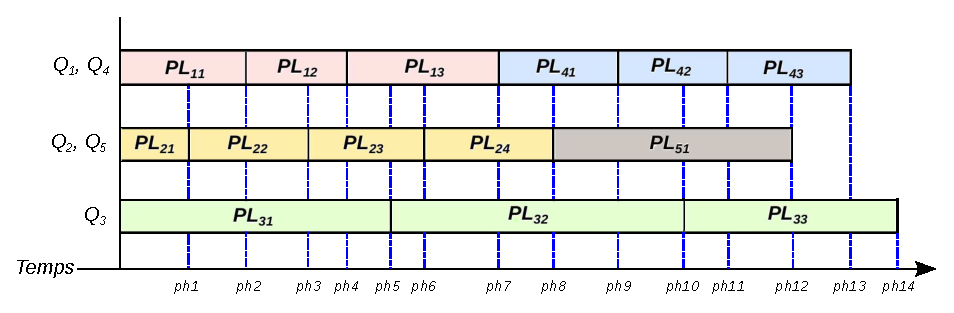
\includegraphics[scale=0.9]{chapitre4/chap4Fig/concurent-pipelines.eps}
 \caption{Les segmentation des pipelines d'une charge de requêtes concurrentes.}
 \label{fig:concurent-pipelines}
\end{figure}

\begin{algorithm}
\caption{Algorithme de prédiction}
\label{algo:prediction-algo}
\begin{algorithmic}[1]
\Require  $W = \{q_1, \cdots, q_n\}$ \Comment{une charge de $n$ requêtes SQL}
\Ensure $P_w$ \Comment{la consommation d'énergie estimée pour la charge $W$}
\ForAll {requête $i \in W$}
    \State $Plan_i \leftarrow GetPlan(i)$;
    \State $PL_i \leftarrow GetPipelines(Plan_i)$;
\EndFor
\State
$PLMixActuel \leftarrow \emptyset$;
\ForAll {requête $i \in W$}
    \State $PLMixActuel \leftarrow PLMixActuel + PL_{i1}$;
\EndFor
\State

\While{$PLMixActuel \neq \emptyset$}
	\State $PL_{ij} \leftarrow PlusCourtPipeline(PLMixActuel)$;
	\State $t_{min} \leftarrow t_{ij}$;
	\State $Co\hat{u}t \leftarrow 0$;
	\ForAll {$PL_{ik} \in CurrentMix$}
		\State $Co\hat{u}t \leftarrow Co\hat{u}t + Co\hat{u}t_{ik} \times \frac{t_{min}}{t_{ik}}$;
	\EndFor
	\State $P_w \leftarrow P_w + EstimePuissance(Co\hat{u}t)$;
	\State Retirer $PL_{ij}$ depuis $MixActuel$;
	\If{$aPlusDePipelines(PL_i)$}
		\State $PLMixActuel \leftarrow PLMixActuel + PL_{i(j+1)}$;
	\EndIf
\EndWhile

\State
\State
\Return $P_w$;
\end{algorithmic}
\end{algorithm}

L'exécution de la charge de requêtes est assimilée à l'exécution d'une suite de mixes de pipeline. L'exécution de chaque mix est appelée une phase de pipeline. Un changement de phase se produit quand un pipeline termine son exécution et un autre pipeline commence. Notre objectif est de déterminer les phases de pipeline et les transitions entre eux et d'estimer la quantité d'énergie consommée par chaque phase. La consommation d'énergie de la charge de requêtes est la consommation totale de toutes les phases. Cette idée est présentée dans l'\ref{algo:prediction-algo}.

Dans cet algorithme, nous générons d'abord le plan d'exécution $Plan_i$ pour chaque requête $Q_i$ en appelant l'optimiseur de requêtes, puis nous créons la segmentation de pipelines $PL_i$ de chaque $Plan_i$. Le premier pipeline $PL_{i1} $ dans chaque $PL_i$ est ajouté au mix en cours d'exécution $CurrentPLMix$. Ensuite, nous continuons l'exécution par phase tant que le mix actuel ne soit pas vide. Nous déterminons le pipeline $PL_{ij} $ avec le temps d'exécution le plus court $t_{min}$. Ensuite, nous calculons \textit{le coût énergétique du travail effectué} par chaque pipeline $PL_{ik} $ dans le mix actuel, en multipliant le coût de chaque pipeline par $\frac{t_{min}}{t_{ik}} $, où $t_{ik}$ est le temps d'exécution du pipeline $PL_{ik}$. Nous appelons la procédure d'estimation d'énergie pour obtenir l'énergie du mix de pipeline actuel, et nous retirons $P_{ij}$ du mix. Si $PL_i$ contient plus de pipelines après la fin d'exécution du $P_{ij}$, nous ajoutons le suivant $P_{i(j+1)}$ dans le mix en cours et nous répétons ce processus jusqu'à ce que toutes les requêtes de la charge sont terminées. La consommation d'énergie finale de la charge de requêtes est la somme de consommation de chaque phase.

\subsection{Modélisation des pipelines}
Après l'identification des paramètres de notre modèle et le niveau de modélisation. La prochaine étape consiste à modéliser ces paramètres. Dans cette section, nous allons donner une formalisation pour notre approche. Ensuite, nous construisons notre modèle en identifiant le modèle mathématique qui décrit notre problème d'estimation d'énergie. Cette phase de construction combine les paramètres identifiés dans les sections précédentes avec une méthode d'apprentissage automatique pour trouver le meilleur modèle (boite grise).

\subsubsection{Coût CPU et E/S des pipelines}
Dans un SGBD traditionnel, le coût d'exécution de la requête est traité comme une combinaison linéaire de trois composantes : le coût du CPU, d'E/S et le coût de la communication \cite{Xu13}. Inspiré par cette méthodologie, nous proposons d'utiliser ces coûts pour modéliser les pipelines des requêtes.
Pour une charge de requête donnée, l'optimiseur de requêtes est responsable de l'estimation des coûts CPU et d'E/S. Notre stratégie pour la modélisation des pipelines est de profiter des modèles de coûts qui sont déjà intégrés dans les SGBD pour l'optimisation des requêtes. Dans un SGBD, pour traiter les tuples, chaque opérateur appartenant à un pipeline doit effectuer des tâches de CPU et/ou d'E/S. Le coût de ces tâches représente le << \textit{coût du pipeline} >>, qui est la puissance d'électricité active censée être consommée afin de terminer les tâches. Dans cette thèse, nous nous concentrons sur une configuration de serveur centralisé et laissons l'étude des BD distribuées pour les futurs travaux. Ainsi, le coût de la communication peut être ignoré. Plus formellement, pour une charge de requête donnée $W$ composée par des requêtes $Q$, notre modèle de coût énergétique pour $W$ est défini comme suit :
\begin{equation}
Puissance(W) = \sum_{i=1}^{n} Puissance(Q_i)
\end{equation}
Soit $Q_i$ une requête composée de $p_i$ pipelines $\{PL_1, PL_2, \dots, PL_p\}$. Le coût de l'énergie $Puissance(Q_i)$ de la requête $Q_i$ est donné par l'équation suivante :
\begin{equation}
Puissance(Q_i) = \frac{\sum_{j=1}^{p} Puissance(PL_j) * Time(PL_j)}{Time(Q_i)}
\end{equation}
$Time(PL_j)$ et $Time(Q_i)$ représentent respectivement, le temps d'exécution du pipeline $j$ et la requête $Q_i$. Ces deux facteurs sont complètement ignorés par Xu \textit{et al.} \cite{Xu13}. Dans notre modèle, le temps est un facteur important pour déterminer le pipeline dominant par les coûts CPU ou E/S dans une requête. Bien que le module statistique du SGBD nous fournisse ces informations, nous allons utiliser le temps d'exécution réel des requêtes afin de tester la qualité de notre modèle.

Notez que le coût d'un pipeline $j$ doit également être décomposé car il peut impliquer plusieurs opérations algébriques. Soit $n_j$ le nombre de ces opérations ($\{OP_1, OP_2, \dots, OP_n\}$). Le coût énergétique $Puissance(PL_j)$ d'un pipeline $j$ est donné par l'équation suivante :
\begin{equation} \label{eq:cost-model}
Puissance({PL_j}) = \beta_{cpu} \times \sum_{k=1}^{n_j} COUT\_CPU_k + \beta_{es} \times  \sum_{k=1}^{n_j} COUT\_ES_k
\end{equation}
Où $\beta_{cpu}$ et $\beta_{es}$ sont les paramètres du modèle (les unités des coûts énergétiques).

Pour une requête donnée, l'optimiseur utilise le plan d'exécution, les estimations de cardinalité et les formules pour les opérateurs afin de générer les valeurs des différents types d'opérations CPU et d'E/S. Il convertit ensuite ces valeurs en temps en utilisant des paramètres spécifiques au système, tels que la vitesse du processeur et la vitesse du transfert E/S. Par conséquent, dans notre modèle, nous prenons les estimations de CPU et d'E/S avant de les convertir en temps.
Les paramètres du système sont calculés à la création de la BD, et pourraient être peu fiables. Suivant les recommandations du fournisseur de SGBD, nous calibrons ces paramètres pour assurer la précision de l'estimation des ressources et  l'optimalité du plan d'exécution.

Le $COUT\_CPU$ est le nombre estimé de \textit{Cycle de CPU} et de \textit{lecture du cache mémoire} nécessaires au SGBD pour l'exécution de l'opérateur spécifié. De même, le $COUT\_ES$ est le nombre estimé d'\textit {E/S} nécessaire au SGBD pour l'exécution de l'opérateur spécifié.

Dans la littérature, l'estimation de ces deux coûts peut se réaliser suivant deux catégories de techniques : (1) techniques basées sur des fonctions analytiques et (2) techniques basées sur l'optimiseur de requêtes du SGBD \cite{Boukhalfa09Phd}. La première catégorie de techniques \cite{Boukorca15, Kerkad12a, Bouchakri11a} définit une fonction analytique pour calculer le coût d'une requête à partir d'un plan d'exécution prédéfini. À chaque opérateur algébrique, une formule qui prend en entrée des paramètres et des statistiques de la BD est utilisée pour le calcul de coût. L'avantage de cette méthode réside dans la facilité et la rapidité de la mise en œuvre et du calcul, mais elle reste limitée par les hypothèses simples et parfois irréalistes. De plus, elle ne garantit pas l'optimalité  du plan de la requête choisie. Par conséquent, cette méthode ne répond pas aux critères régissant la construction d'un modèle de coût énergétique de qualité, qui ont été décrits dans la \ref{sec:PourquoiModelCout}.

La deuxième catégorie de techniques \cite{Bruno11, Chaudhuri97, Chaudhuri98} fait appel à l'optimiseur de requête du SGBD utilisé pour estimer le coût d'une requête. L'optimiseur évalue les différents plans d'exécution de la requête et retourne l'optimal avec son coût. Le plan et le coût sont fiables comme exigé par nos critères de modélisation. De plus, cette technique rend l'intégration de notre modèle dans un SGBD réel plus facile.

Dans le cadre de cette thèse, nous adaptons une technique appartenant à la deuxième catégorie. Comme indiqué précédemment, en utilisant les coûts CPU et E/S retournés par le SGBD, nous ne dépendons pas du type ou de l'implémentation des opérateurs SQL comme dans \cite{Xu13}. Par conséquent, notre modèle est portable et peut traiter des requêtes plus complexes comme celles du benchmark TPC-DS.

\subsubsection{Estimation des paramètres du modèle}
Le principal défi dans la résolution de l'\ref{eq:cost-model} est de trouver les paramètres du modèle $\beta_{cpu}$ et $\beta_{es}$. Notre méthodologie utilise la technique de régression pour calculer ces paramètres de coût.

La notion de régression est fondamentale dans toutes les sciences appliquées, elle consiste à analyser une relation entre deux variables quantitatives et à l'exploiter pour estimer la valeur inconnue de l'une à l'aide de la valeur connue de l'autre. Elle est couramment utilisée dans les techniques de gestion et de commercialisation, pour expliquer un chiffre d'affaires en fonction des dépenses publicitaires, effectuer des prévisions de bénéfices, de ventes, etc. Dans les sections suivantes, nous détaillons cette technique, et nous formalisons la démarche utilisée pour calculer les paramètres de notre modèle de coût.

\paragraph{Régression linéaire}
On étudie en régression deux variables quantitatives, dont l'une appelée variable \textit{expliquée}, est considérée comme \textit{dépendante} de l'autre, appelée variable \textit{explicative} ou \textit{indépendante}. On note habituellement la variable expliquée $Y$, et la variable explicative $X$. Un exemple de cette dépendance est lorsqu'on mesure la consommation d'une voiture à des vitesses choisies pour établir la relation entre la consommation (variable dépendante) et la vitesse (variable indépendante) \cite{Montgomery12, Neter96, Kutner04}.

On qualifie un modèle de régression de \textit{simple} lorsque qu'il y a une seule variable explicative. \`A l'inverse, on le qualifie de \textit{multiple} en présence d'au moins de deux variables explicatives. Le modèle de régression simple est une équation censée représenter cette relation entre les deux variables. Il s'écrit sous cette forme :
\begin{equation}
Y = f(X) + \epsilon
\end{equation}
La variable $Y$ est supposée être approximativement égale à une fonction $f$ de $X$, le terme $\epsilon$ caractérisant la marge d'erreur ou d'imprécision du modèle. L'objectif est de préciser la nature de la régression (la fonction $f$), de mesurer le degré d'imprécision (le terme $\epsilon$), de détecter les observations qui ne suivent pas le modèle et d'effectuer des prévisions de $Y$ pour différentes valeurs de $X$. Nous supposons d'abord que la nature de la liaison entre les deux variables est linéaire. Le modèle de régression s'exprime alors de la façon suivante :
\begin{equation}
y = \beta x + a + \epsilon
\end{equation}
Où $\beta$ et $a$ représentent les coefficients théoriques de la régression et leurs valeurs sont inconnues. L'estimation de ces coefficients peut se faire avec plusieurs méthodes. Parmi les méthodes les plus utilisées on trouve la méthode des moindres carrés.

\subparagraph{Critère des moindres carrés}
Supposons que les données de l'étude de la régression se présentent sous la forme d'une suite de $n$ couples $[x(i), y(i)]$, numérotés de $i = 1$ à $i = n$. Nous avons représenté sur la \ref{fig:least-squares} cet ensemble de données. L'objectif est de déterminer les coefficients de la droite $y = \beta x + a$, appelée \textit{droite de régression}, la plus proche possible des $n$ points.

\begin{figure}
 \centering
 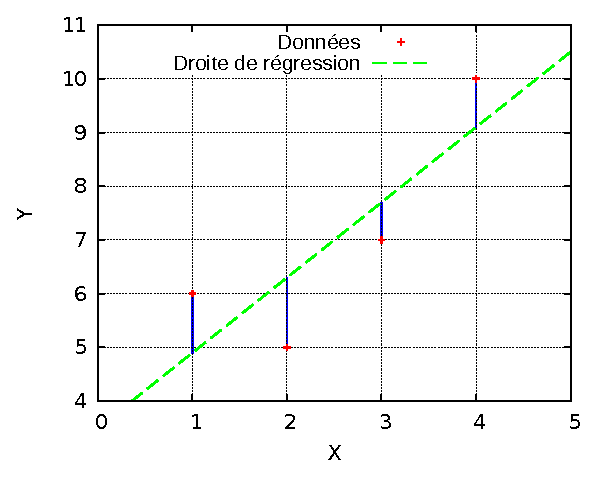
\includegraphics[scale=1.0]{chapitre4/chap4Fig/least-squares.eps}
 \caption{La régression linéaire par la méthode des moindres carrés.}
 \label{fig:least-squares}
\end{figure}

Plus précisément, il s'agit de reconstruire le mieux possible la variable $Y$ en fonction de la variable $X$ et de déterminer la droite de façon à ce que les termes d'erreur de la forme $\epsilon(i) = y(i) - [\beta x(i) + a ]$ soient les plus petits possible (les plus proches de 0). Ces termes $e(i)$ sont appelées aussi \textit{résidus}. Pour mesurer la proximité de la valeur 0 à ces erreurs, on cherche les coefficients $\beta$ et $a$ tel que la somme des carrés de ces termes soit minimale. Ces sommes sont représentées sur la \ref{fig:least-squares} par les longueurs des segments de couleur bleu.

%\begin{theorem}
Les estimations des coefficients de régression théoriques $\beta$ et $a$ sont telles que la somme des carrés des erreurs soit la plus petite possible. Elles sont données par les formules ci-dessous \cite{Neter96} :
 \begin{equation}
 \begin{aligned}
  %\beta = \frac{cov(x,y)}{S_{x}^{2}} = r(x,y) \frac{S_y}{S_x} \\
  \beta = \frac{ \sum_{i=1}^{n}(x_i-\bar{x})(y_i-\bar{y}) }{ \sum_{i=1}^{n} (x_i-\bar{x})^2} \; \text{et} \; a = \bar{y} - \beta \bar{x} \\
  \text{avec : } \; \bar{x} = \frac{1}{n} \sum_{i=1}^{n} x_i \; \text{et} \; \bar{y} = \frac{1}{n} \sum_{i=1}^{n} y_i
  \end{aligned}
 \end{equation}
%\end{theorem}

\subparagraph{Modèle énergétique en régression linéaire}
Appliquant les techniques expliquées dans les sections précédentes sur notre modèle de coût, le coût de l'énergie $Puissance_{PL_j} $ du pipeline $p_j$, avec une relation linéaire entre les paramètres du modèle, est calculé comme suit :
\begin{equation} \label{eq:lin-reg-equation}
Puissance(PL_j) = \beta_0 + \beta_1 \times COUT\_ES+ \beta_2 \times COUT\_CPU + \epsilon
\end{equation}
où $COUT\_ES$, $COUT\_CPU$ désignent les coûts CPU et E/S du pipeline, respectivement. Ces coûts sont fournis par le module de statistiques SGBD, et $\epsilon_i$ est un terme d'erreur ou perturbation, qui représente les erreurs de mesure. Les paramètres $\beta$ sont des coefficients de régression qui seront estimés, tout en apprenant le modèle à partir de données d'apprentissage. Ainsi, les modèles de régression linéaire sont résolus par l'estimation des paramètres du modèle $\beta$, et cela se fait par trouver la solution des moindres carrés. %\cite{McCullough11}.

Nous avons commencé simplement par une régression linéaire avec la formule ci-dessus (\ref{eq:lin-reg-equation}), comme déjà fait dans \cite{Xu13, Kunjir12, Lang11}. Malheureusement, ce modèle ne donne pas de meilleurs résultats surtout quand la taille des données change. En effet, la relation entre la taille des données et la puissance d'électricité n'est pas linéaire. En d'autres termes, le traitement de gros fichiers ne se traduit pas \textit{toujours} par une forte consommation d'énergie. Cela dépend plutôt du type de pipeline (dominé par CPU ou E/S) dans la requête et de son temps d'exécution. Par conséquent, nous avons décidé d'utiliser le modèle de régression polynomiale.

\paragraph{Régression polynomiale}
La régression polynomiale est une analyse statistique qui décrit la variation d'une variable expliquée $y$, en fonction d'une variable explicative $x$. On cherche, par régression, à lier les variables par un polynôme de degré $p$. Le modèle est de la forme \cite{Kutner04} :
\begin{equation}
y = \beta_0 + \beta_1 x + \beta_2 x^2 + \cdots + \beta_p x^p + \epsilon
\end{equation}
Pour simplifier les notations, nous introduisons une variable explicative supplémentaire $x_0$, qui est constante et égale à 1. On peut alors écrire :
\begin{equation}
y = \sum_{j=0}^{p} \beta_j x^j + \epsilon
\end{equation}
Soit, pour chaque unité statistique :
\begin{equation}
y(i) = \sum_{j=0}^{p} \beta_j x^j(i) + \epsilon(i)
\end{equation}
Le critère utilisé pour calculer les estimations $\beta_j$ est le même que précédemment : on cherche les valeurs $\beta_0, \beta_1, \cdots, \beta_j, \cdots, \beta_p$ tel que l'ajustement soit le meilleur possible au sens des moindres carrés. On minimise donc la somme $S$ :
\begin{equation}
S = \sum_{i=0}^{n} [ y(i) - \sum_{j=0}^{p} \beta_j x^j(i) ]^2
\end{equation}
La régression polynomiale est considérée comme un cas particulier de la régression linéaire multiple. Cette technique convient quand il y a une relation \textit{non linéaire} entre les variables indépendants et la variable dépendante \cite{Neter96}.

\subparagraph{Modèle énergétique en régression polynomiale}
Nous avons utilisé la régression polynomiale dans notre modèle. Selon nos expérimentations, l'ordre \textit{p=2} nous donne les meilleurs résultats (la somme des carrés des résidus est la plus petite). Le modèle de régression polynomiale avec le degré \textit{p=2} est exprimé comme suit :
\begin{equation} \label{eq:poly-reg-equation}
\begin{aligned}
  Puissance(PL_j) = \beta_{0} + \beta_{1} \times (COUT\_ES) + \beta_{2} \times (COUT\_CPU) + \\
  \beta_{3} \times (COUT\_ES^2) + \beta_{4} \times (COUT\_CPU^2) + \beta_{5} \times (COUT\_ES \times COUT\_CPU) + \epsilon
\end{aligned}
\end{equation}
Les résultats de cette méthode sont beaucoup plus véridiques qu'une régression linéaire.

\subsubsection{Apprentissage}
Comme mentionné ci-dessus, les paramètres $\beta$ sont estimés tout en apprenant le modèle à partir de données d'apprentissage.
Ensuite, nous effectuons des séries d'observations où les requêtes sont bien choisies et les valeurs de l'énergie consommée par le système sont récupérées au moyen  d'un équipement de mesure lors de l'exécution de ces requêtes. En même temps, pour chaque instance d'apprentissage, nous segmentons les opérateurs de requête en un ensemble de pipelines, et nous calculons leurs coûts.

\paragraph{Données d'apprentissage}
Pour générer des données d'apprentissage, nous avons créé notre charge de requête personnalisée basé sur les données du benchmark TPC-H (au facteur d'échelle 10 et 100). La charge contenant 110 requêtes est caractérisée par (i) des requêtes ayant des opérations qui épuisent le processeur du système (requêtes gourmandes en CPU) et (ii) des requêtes avec des opérations qui épuisent les ressources de stockage (requêtes gourmandes en E/S). Pour ce faire et en s'inspirant des travaux précédents \cite{Kunjir12}, nous varions d'une requête à une autre : le nombre de tables à lire, le nombre/type des prédicats de jointure, le nombre des opérations du tri/regroupement, le type des fonctions d'agrégation allant de la plus simple (\texttt{count(*)}) à des fonctions plus complexes. L'ensemble de requête interrogeant des données de 10 Go de taille est présenté dans l'\ref{annex:TrainQueries} (page \pageref{annex:TrainQueries}).

Nous notons que pour le coût de CPU de certaines requêtes, en particulier celles contenant des agrégations et des fonctions analytiques, n'est pas calculé par le SGBD malgré la puissance intensive consommée par ces deux types de fonctions. Pour surmonter cette contrainte, nous proposons de calculer \textit{manuellement} les cycles de CPU requis pour exécuter ces fonctions d'agrégation, en utilisant les coûts de notre machine pour faire les instructions de base telles que \textit{ADD, SUB, MUL, DIV} et \textit{COMPARE} \cite{IntelOptimize14}. Les estimations obtenues sont ensuite multipliées par le nombre de lignes.

\paragraph{Régression avec le logiciel R}
Après avoir collecté la consommation de puissance, les coûts CPU et E/S des requêtes d'apprentissage, nous appliquons l'équation de régression \eqref{eq:poly-reg-equation} pour trouver les paramètres du modèle et ainsi décrire le comportement des pipelines vis-à-vis de la consommation de l'énergie. Finalement, après l'extraction des paramètres, nous pouvons estimer la puissance des nouvelles requêtes sans avoir à utiliser les équipements de mesure.

Nous décrivons dans cette section la mise en œuvre de la régression à l'aide de R\footnote{http://www.r-project.org/}. R est un logiciel libre et gratuit et un langage d'analyse statistique et graphique \cite{Ihaka96} brassant de nombreuses fonctions traitant la modélisation linéaire et non linéaire, la statistique multivariée, l'analyse de séries chronologiques, la classification, le clustering, etc.

Pour notre problème de régression, R dispose de la commande \texttt{lm()}, qui signifie \textit{linear model} ou modèle linéaire, permettant d'obtenir l'équation de la droite de régression. La lecture de données, l'application de la régression et l'affichage de résultat peut être réalisé de la manière présentée dans la \ref{fig:reg-lin-r}.

\begin{figure}
%\lstinputlisting[language=R]{chapitre4/chap4Fig/reg-lin.r}
\begin{lstlisting}[language=R]
> data <- read.csv('energy-data.csv', comment.char = "#", sep='\t')
> result <- lm(Power ~ IO + CPU, data=data)
> summary(result)
Call:
lm(formula = Power ~ IO + CPU, data = data)

Residuals:
    Min      1Q  Median      3Q     Max 
-2.7331 -0.5331 -0.0666  0.1971  6.5852 

Coefficients:
              Estimate Std. Error t value Pr(>|t|)    
(Intercept)  3.878e+01  1.824e-01  212.63   <2e-16 ***
IO          -2.891e-07  2.623e-08  -11.02   <2e-16 ***
CPU          3.722e-12  2.327e-13   15.99   <2e-16 ***
---
Signif. codes:  0 '***' 0.001 '**' 0.01 '*' 0.05 '.' 0.1 ' ' 1

Residual standard error: 1.436 on 139 degrees of freedom
Multiple R-squared:  0.6656,    Adjusted R-squared:  0.6608 
F-statistic: 138.3 on 2 and 139 DF,  p-value: < 2.2e-16
\end{lstlisting}
  \caption{Exemple d'une régression linéaire avec le logiciel R.}\label{fig:reg-lin-r}
\end{figure}

Le \texttt{Intercept} correspond ici à $\beta_0$ de notre \ref{eq:lin-reg-equation} et le $IO$, $CPU$ correspondent respectivement au $\beta_1$, $\beta_2$  de notre équation. Les valeurs de ces termes sont dans la colonne \texttt{Estimate}. L'équation de droite de régression est donc :
\begin{equation}
 Puissance(PL_j) = 38,78 - 2,891 \times 10^{-7} \times COUT\_ES + 3,722 \times 10^{-12} \times COUT\_CPU
\end{equation}

La commande \texttt{summary()} affiche également d'autres informations sur le modèle, tel que les valeurs de résidus, l'erreur standard, le coefficient de détermination, etc. De même pour la régression polynomiale de degré 2, on utilise la commande présentée dans la \ref{fig:reg-poly-r} suivante.

\begin{figure}
%\begin{verbatim}
\begin{lstlisting}[language=R]
> result <- lm(Power ~ poly(IO, CPU, degree=2, raw=TRUE), data=data)
> summary(result)

Call:
lm(formula = Power ~ poly(IO, CPU, degree = 2, raw = TRUE), data = data)

Residuals:
    Min      1Q  Median      3Q     Max 
-2.3579 -0.3407  0.0850  0.3690  4.0238 

Coefficients:
                                           Estimate Std. Error t value Pr(>|t|)
(Intercept)                               3.841e+01  1.946e-01 197.378  < 2e-16
poly(IO, CPU, degree = 2, raw = TRUE)1.0 -1.281e-06  1.851e-07  -6.922 1.60e-10
poly(IO, CPU, degree = 2, raw = TRUE)2.0  9.026e-14  1.532e-14   5.892 2.85e-08
poly(IO, CPU, degree = 2, raw = TRUE)0.1  2.934e-11  1.652e-12  17.763  < 2e-16
poly(IO, CPU, degree = 2, raw = TRUE)1.1 -2.236e-18  1.561e-19 -14.319  < 2e-16
poly(IO, CPU, degree = 2, raw = TRUE)0.2 -2.663e-25  1.575e-25  -1.691   0.0931
...
\end{lstlisting}
  \caption{Exemple d'une régression polynomiale avec le logiciel R.}\label{fig:reg-poly-r}
\end{figure}

On obtient les mêmes sorties comme pour la commande précédente. L'équation de la droite de régression dans ce cas est :
\begin{equation}
\begin{aligned}
Puissance(PL_j) = 38,41 - 1,281 \times 10^{-6} COUT\_ES + 2,943 \times 10^{-11} COUT\_CPU \\
+ 9,026 \times 10^{-14} COUT\_ES^2 -2,663 \times 10^{-25} COUT\_CPU^2 \\
-2,236 \times 10^{-19} COUT\_ES \times COUT\_CPU \\
\end{aligned}
\end{equation}

\subsection{Méthode d'évaluation}
Nous élaborons une phase de test où le coût d'énergie estimé \textit{(E)} par notre modèle est comparé avec la consommation d'énergie réelle \textit{(M)} du système, relevée à l'aide des équipements de mesure d'énergie. Pour quantifier la précision du modèle, nous avons utilisé la métrique du taux d'erreur suivante pour une seule requête :
\begin{equation}
 Erreur = \frac{|M - E|}{M}
\end{equation}

Et pour une charge de $n$ requêtes, nous avons utilisé la métrique d'erreur moyenne et maximale suivantes : %DONE: revisite max_error formula !
\begin{equation}
\begin{aligned}
 Erreur_{moy} = \frac{1}{n} \times \sum_{i=1}^{n} \frac{|M_i - E_i|}{M_i} \\
 Erreur_{max} = Max (\frac{|M - E|}{M})
\end{aligned}
\end{equation}

La \ref{fig:power-model} résume les étapes de notre approche composée de trois étapes.  Nous avons d'abord identifié le niveau de modélisation le plus adéquat comme étant les pipelines et les paramètres du modèle comme étant le coût E/S et CPU. Dans l'étape de construction du modèle, la méthode choisie est la régression polynomiale. Finalement, l'étape de validation permet d'estimer l'énergie d'une requête sans recourir à l'équipement de mesure et intégrer le modèle validé dans une structure d'optimisation afin de minimiser la consommation d'énergie dans les BD. 

\begin{figure}
 \centering
 \includegraphics[scale=0.80]{chapitre4/chap4Fig/costmodel-methodology-final.pdf} % power-model.eps
 \caption{Vue d'ensemble sur le modèle de coût énergétique.}
 \label{fig:power-model}
\end{figure}

\section{Évaluation de notre modèle de coût}\label{sec:experiment}
Dans cette section, nous présentons des résultats expérimentaux montrant l'efficacité de notre modèle proposé. Nous décrivons d'abord l'architecture et le jeu de données d'expérimentations, puis nous évaluons la performance de notre modèle d'estimation d'énergie.

\subsection{Architecture d'expérimentations}
Pour mesurer la consommation réelle d'énergie, nous avons créé une configuration similaire aux travaux précédents \cite{Rodriguez11, Xu10b, Kunjir12} que nous utilisons même dans le reste de nos expérimentations présentées dans les prochains chapitres. Cette configuration utilise le multimètre << \textit{Watts UP? Pro ES} >> \footnote{https://www.wattsupmeters.com/} qui a une résolution maximale d'une seconde.
Le dispositif est directement connecté entre la prise d'alimentation et la station de travail sur laquelle la BD est déployée. Cet ordre permet de mesurer la consommation d'énergie globale de la station de travail. Les valeurs mesurées sont enregistrées et traitées dans une machine de contrôle séparée connectée avec le multimètre via un câble USB.
% \begin{figure}
%  \centering
%  \includegraphics[scale=0.6]{chapitre4/chap4Fig/schema.png}
%  \caption{Architecture d'expérimentations.}
%  \label{fig:arch-setup}
% \end{figure}

Nous avons utilisé une station de travail Dell PowerEdge R210 II ayant un processeur Intel Xeon E3-1230 V2 de 3.30GHz, 10 Go de mémoire DDR3 et une configuration disque dur de 2x500 Go. A noter que des techniques comme la \textit{tension-fréquence dynamique du processeur} (DVFS) ne sont pas appliquées dans nos expérimentations. Nous répétons chaque expérience plusieurs fois pour assurer la confiance dans les valeurs observées.

Notre station de travail est installée avec la dernière version du SGBD Oracle 11gR2 sous Ubuntu Server 14.04 LTS avec noyau Linux 3.13. Afin de minimiser les influences indésirables, nous avons désactivé les tâches de fond inutiles et vidé le cache du système et le buffer d'Oracle avant chaque exécution de requête.

\subsubsection{Exécution des requêtes et capture d'énergie}

\begin{figure}
 \centering
 \includegraphics[scale=0.7]{chapitre4/chap4Fig/experiment-setup.pdf}
 \caption{Applications de gestion d'expérimentations.}
 \label{fig:experiment-setup}
\end{figure}

Pour réaliser nos expérimentations, nous avons développé une application et un script pour automatiser le processus des tests. La \ref{fig:experiment-setup} représente l'architecture logicielle des expérimentations. Une application client/serveur basée sur les sockets et implémentée en langage C est mise en œuvre. La machine de contrôle contient la partie serveur de l'application dont les tâches se résument à :
\begin{enumerate}
 \item l'établissement d'une connexion via le réseau avec la station de travail ;
 \item le lancement/l'arrêt des expérimentations ;
 \item l'enregistrement des valeurs d'énergie via le multimètre en invoquant son pilote.
\end{enumerate}

La station de travail contient la partie client de l'application  et ses tâches consistent à :
\begin{enumerate}
 \item l'établissement de la connexion avec l'application serveur ;
 \item le vidage du cache de la BD à l'aide des commandes Oracle suivantes:
 \begin{lstlisting}[language=sql]
-- Clean the cache
ALTER SYSTEM FLUSH SHARED_POOL;
ALTER SYSTEM FLUSH BUFFER_CACHE;
\end{lstlisting}
 \item le vidage du cache du système d'exploitation à l'aide du script \textit{shell} suivant :
 \begin{lstlisting}[language=bash]
#!/bin/bash
# To free pagecache, dentries and inodes (linux kernel)
sync && echo 3 | tee /proc/sys/vm/drop_caches
\end{lstlisting}
 \item la connexion avec le SGBD ;
 \item le lancement et la gestion d'ordonnancement de requêtes d'apprentissage et de tests ;
 \item l'extraction du plan d'exécution avec tous ses informations (coût d'E/S et de CPU, temps d'exécution des opérateurs, etc.), à l'aide de la commande Oracle suivante :
 \begin{lstlisting}[language=sql]
SELECT DBMS_SQLTUNE.report_sql_monitor(
  sql_id       => '526mvccm5nfy4',
  type         => 'ACTIVE',
  report_level => 'ALL') AS report
FROM dual;
\end{lstlisting}
\end{enumerate}

\subsection{Jeu de données}
Dans les expérimentations, nous utilisons les jeux de données et les requêtes issues des deux benchmarks TPC-H et TPC-DS \cite{TPCH, TPCDS}, interrogeant des données de 10 Go et de 100 Go de taille (facteur d'échelle). Le TPC-H est un benchmark décisionnel conçu pour le requêtage ad-hoc où les requêtes ne sont pas connues à l'avance. Le schéma modélise un modèle produits-commandes-fournisseurs contenant 2 tables de faits et 6 tables de dimensions (cf. \ref{fig:tpch-schema}), avec une charge de 22 requêtes décisionnelles caractérisées par un large volume de données et un degré élevé de complexité.
TPC-DS qui est le successeur annoncé de TPC-H, modélise un entrepôt de données. Le schéma de TPC-DS représente les fonctions décisionnelles d'un détaillant sous la forme de plusieurs schémas en flocon de neige. Il comprend 17 dimensions partagées par 7 tables de faits, ce qui le transforme en un schéma en constellation. Le \ref{tab:tpcds-table-rows} représente le nombre de lignes dans les tables de faits avec une taille de 100 Go (facteur d'échelle = 100). La charge de requêtes de TPC-DS est composée de 99 requêtes et  constituée de quatre classes de requêtes : requêtes de rapports, requêtes décisionnelles ad-hoc, requêtes de traitement analytique en ligne (On-Line Analytical Processing, OLAP) et requêtes d'exploration de données \cite{Nambiar06}.
\begin{figure}
 \centering
 \includegraphics[scale=0.6]{chapitre4/chap4Fig/tpch-schema.pdf}
 \caption{Schéma du benchmark TPC-H.}
 \label{fig:tpch-schema}
\end{figure}

\begin{table}[]
\centering
\caption {Cardinalité des tables de faits du benchmark TPC-DS avec une taille de 100 Go.}\label{tab:tpcds-table-rows}
%\rowcolors{0}{}{lightgray}
\begin{tabular}{ll}
\toprule
\textbf{Table} & \textbf{Cardinalité} \\ \midrule
	store\_sales & 288 millions \\ 
	store\_returns & 28,8 millions \\ 
	catalog\_sales & 144 millions \\
	catalog\_returns & 14,4 millions \\
	web\_sales & 72 millions \\
	web\_returns & 7,2 millions \\
	inventory & 400 millions \\ \bottomrule
\end{tabular}
\end{table}

L'ensemble des données et de requêtes des deux benchmarks ont été générés avec l'outil \texttt{dbgen} fourni par le TPC. Une fois les données générées, des scripts sont utilisés pour peupler la BD à l'aide du l'outil \texttt{sqlloader} fourni par Oracle.
Dans le cas d'exécution des requêtes en mode isolé, chaque charge contient une seule requête (une seule requête est en exécution par le SGBD à un instant donné).
Dans le cas du mode concurrent, nous avons varié le taux de multiprogrammation (MPL $\in \{2,\cdots,10,13,15\}$).

\subsection{Résultats pour une requête isolée}
Comme décrit dans la section précédente, notre modèle de coût est composé de deux parties : les paramètres d'énergie qui peuvent être calculés par le biais d'une procédure d'apprentissage, et les paramètres de pipeline (p. ex. les coûts CPU et E/S) qui peuvent être lus à partir des statistiques de BD déjà disponibles. Dans cette section, nous présentons les résultats de ces deux étapes.

\subsubsection{Résultat d'apprentissage}
Dans la phase d'apprentissage, nous collectons à chaque exécution de requête, des statistiques relatives à l'exécution des pipelines et à la consommation d'énergie du système. Ces données collectées sont utilisées par le logiciel R pour trouver les meilleures valeurs des paramètres du modèle. Sur la base des résultats obtenus, une preuve probabiliste pour démontrer les bornes de confiance de notre modèle et des résultats est donnée dans l'\ref{annex:ConfidenceBounds} (page \pageref{annex:ConfidenceBounds}).

Les résultats de la phase d'apprentissage pour les valeurs retournées par le modèle linéaire et polynomiale (l'\ref{eq:lin-reg-equation} et l'\ref{eq:poly-reg-equation}) sont tracés dans la \ref{fig:tpch-reg}.

\begin{figure}
  \centering
  \subfloat[Modèle de régression linéaire\label{fig:tpch-reg-lin}]{
    \centering
    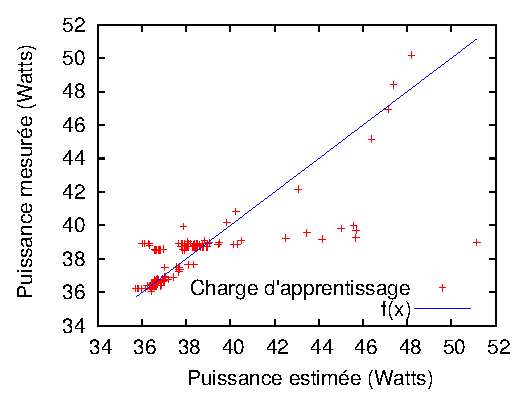
\includegraphics[width=0.45\textwidth]{chapitre4/chap4Fig/tpch-reg-lin.eps}
  }
  \quad
  \subfloat[Modèle de régression polynomiale\label{fig:tpch-reg-poly}]{
    \centering
    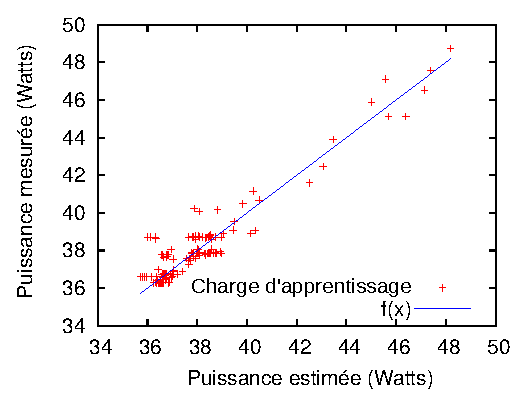
\includegraphics[width=0.45\textwidth]{chapitre4/chap4Fig/tpch-reg-poly.eps}
  }
  \caption{La qualité des méthodes de régressions pour la phase d'apprentissage du modèle de coût énergétique.}\label{fig:tpch-reg}
\end{figure}

Comme nous pouvons le voir sur la \ref{fig:tpch-reg-lin}, il existe des différences significatives entre la consommation d'énergie estimée et réelle pour de nombreuses requêtes. Néanmoins, la consommation d'énergie estimée et réelle rapprochent de près les lignes diagonales lors de l'utilisation d'une régression polynomiale (\ref{fig:tpch-reg-poly}).
% cela justifie notre choix d'utiliser une régression polynomiale

\subsubsection{Résultat avec TPC-H}
Pour tester notre modèle avec un grand ensemble de données, nous exécutons tous les 22 requêtes du benchmark TPC-H avec une taille de deux facteurs d'échelle, 10 Go et 100 Go. Nous notons que la plupart des requêtes contiennent plus de 4 pipelines.
Les résultats sont présentés dans le \ref{tab:tpch-results}.

\begin{table}[]
\centering
\caption {Erreurs d'estimation d'énergie dans les requêtes du benchmark TPC-H avec différentes tailles de BD.}\label{tab:tpch-results}
%\rowcolors{5}{}{lightgray}
\begin{tabular}{cccccc}
\toprule
\multirow{2}{*}{\textbf{Requête}} & \multicolumn{2}{c}{\textbf{Erreur (\%)}} & \multirow{2}{*}{\textbf{Requête}} & \multicolumn{2}{c}{\textbf{Erreur (\%)}} \\ \cmidrule(lr){2-3} \cmidrule(l){5-6} 
    & \textbf{10 Go} & \textbf{100 Go} & & \textbf{10 Go} & \textbf{100 Go} \\ \midrule
	$Q1$ & 1,2 & 0,9 & $Q12$ & 1,9 & 0,05 \\ 
	$Q2$ & 10,1 & 8,9 & $Q13$ & 12,8 & 6,1 \\ 
	$Q3$ & 1,0 & 0,1 & $Q14$ & 0,4 & 0,6 \\ 
	$Q4$ & 0,5 & 0,3 & $Q15$ & 2,3 & 1,0 \\ 
	$Q5$ & 1,2 & 0,6 & $Q16$ & 0,4 & 1,7 \\ 
	$Q6$ & 1,3 & 0,1 & $Q17$ & 0,2 & 1,4 \\ 
	$Q7$ & 1,1 & 0,7 & $Q18$ & 1,9 & 3,7 \\ 
	$Q8$ & 0,5 & 0,1 & $Q19$ & 0,6 & 1,0 \\ 
	$Q9$ & 1,9 & 0,8 & $Q20$ & 1,8 & 2,1 \\ 
	$Q10$ & 0,6 & 1,2 & $Q21$ & 0,9 & 0,4 \\ 
	$Q11$ & 4,8 & 0,3 & $Q22$ & 0,007 & 2,1 \\ \bottomrule
\end{tabular}
\end{table}

Comme nous pouvons le voir dans le tableau, l'erreur moyenne est généralement très minimale (1,6\% pour l'ensemble de données de 10 Go et 2,1\% pour celui de 100 Go), et l'erreur maximale est habituellement au-dessous de 5\%. Les plus grandes erreurs dans les estimations faites par notre modèle de coût (p. ex. \textit{Q2} et \textit{Q13}) sont dues à des erreurs d'estimation de cardinalité faite par l'optimiseur de requêtes.

Par exemple, le troisième pipeline de \textit{Q2} de l'ensemble de données de 100 Go est le plus long pipeline dans la requête. Le nombre estimé de lignes est de seulement 180 692 lignes tandis que le nombre réel de lignes est de 1 362 975. Ainsi, les valeurs des coûts de CPU et de E/S sont systématiquement fausses. Puisque notre étude dans ce stade traite les SGBD comme une << boîte noire >>, nous ne pouvons pas vérifier le modèle basé sur des cardinalités réelles qui sont obtenues après l'exécution de la requête.

\subsubsection{Résultat avec un schéma complexe : TPC-DS}
Pour vérifier la portabilité du modèle sur un nouveau schéma de BD, nous avons pris le benchmark TPC-DS qui est plus complexe que le benchmark TPC-H en raison de son schéma diverse, sa distribution de données et sa charge de requête d'aide à la décision. Nous avons utilisé une BD d'une taille de 100 Go.

Motivé par \cite{Poess07}, nous avons sélectionné 16 requêtes sur les 99 requêtes, en veillant à ce que les deux types soient présents (requêtes gourmandes en CPU et/ou en E/S). Le nombre moyen des pipelines est 7. La \ref{fig:tpcds-100-set1-power} montre les résultats d'expérimentation. On constate que l'erreur des prédictions du modèle est inférieure à 10\%. De même, nous observons la présence d'une seule requête avec une erreur importante, à savoir la \textit{Q47}. En analysant la structure de cette requête, nous avons constaté que l'erreur vient du fait que le coût de la fonction analytique \texttt{rank()} n'est pas donné par le SGBD. Pour le vérifier, nous avons supprimé la partie de code SQL contenant la fonction \texttt{rank()} dans \textit{Q47} et nous l'avons renommée et exécutée sous le nom de \textit{Q47p}. Comme nous pouvons le voir dans la \ref{fig:tpcds-100-set1-power}, l'erreur d'estimation est descendue à 7,5\%.

Cette situation (calcul du coût des agrégations et des fonctions d'analyse) doit être considérée par les vendeurs de SGBD pour faciliter le développement de BD énergétique, comme précédemment souligné dans \cite{Harizopoulos09, Graefe08}.

\begin{figure}
 \centering
 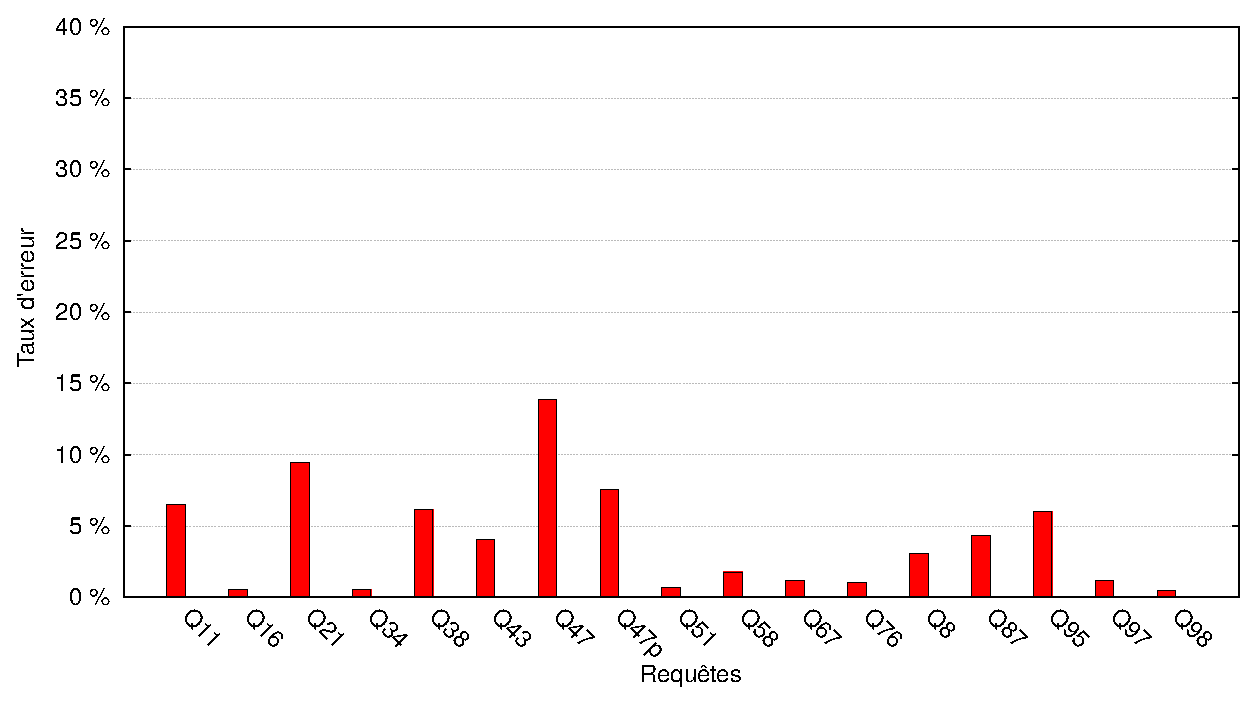
\includegraphics[scale=0.5]{chapitre4/chap4Fig/tpcds-100-set1-error.eps}
 \caption{Erreurs d'estimation d'énergie dans les requêtes du benchmark TPC-DS.}
 \label{fig:tpcds-100-set1-power}
\end{figure}

\subsubsection{Résultat avec une nouvelle configuration matérielle}
Dans un autre test, nous avons réduit la mémoire de BD à 2 Go et exécuté la charge de requêtes du TPC-H. Les résultats sont présentés dans le \ref{tab:tpch-2ram-results}.
Dans ce scénario, lorsque les résultats intermédiaires des opérateurs (comme la phase de construction de la table de hachage ou de tri externe) ne peuvent pas tenir dans la mémoire disponible, le SGBD va les enregistrer sur le disque. Cela conduit à plus d'E/S et un changement de comportement de consommation d'énergie. L'expérience montre que l'erreur d'estimation moyenne est de 2,5\%. Ainsi, notre modèle peut faire face à cette situation.

\begin{table}[]
\centering
\caption {Erreurs d'estimation d'énergie dans les requêtes du benchmark TPC-H avec 2 Go de mémoire.}\label{tab:tpch-2ram-results}
%\rowcolors{0}{}{lightgray}
\begin{tabular}{cccc}
\toprule
\textbf{Requête} & \textbf{Erreur 10 Go (\%)} & \textbf{Requête} & \textbf{Erreur 10 Go (\%)} \\ \midrule
	$Q1$ & 1,4 & $Q12$ & 0,8 \\ 
	$Q2$ & 11,9 & $Q13$ & 4,2 \\ 
	$Q3$ & 1,4 & $Q14$ & 1,7 \\
	$Q4$ & 0,7 & $Q15$ & 1,9 \\
	$Q5$ & 2,4 & $Q16$ & 2,4 \\
	$Q6$ & 1,5 & $Q17$ & 0,8 \\ 
	$Q7$ & 2,7 & $Q18$ & 6,5 \\
	$Q8$ & 1,5 & $Q19$ & 0,0 \\ 
	$Q9$ & 2,2 & $Q20$ & 0,3 \\ 
	$Q10$ & 2,7 & $Q21$ & 2,3 \\
	$Q11$ & 5,6 & $Q22$ & 0,07 \\ \bottomrule
\end{tabular}
\end{table}

\subsubsection{Résultat avec un nouveau SGBD}
Dans ces expérimentations, nous avons à la fois changé le SGBD et le matériel de déploiement  pour voir la robustesse de notre modèle. Précisément, nous avons utilisé le SGBD libre PostgreSQL en version 9.4.5, et comme matériel, nous avons utilisé une station de travail Dell PowerEdge R310 ayant un processeur Xeon X3430 de 2,40 GHz et 32 Go de mémoire DDR3. Pour la BD, nous avons utilisé le même benchmark TPC-H avec un facteur d'échelle de 10 et de 100 Go.
Les résultats de l'exécution de la charge de requêtes sont présentés dans le \ref{tab:tpch-results-postgres}.
Nous notons que certaines requêtes ont été interrompues car elles dépassent les 72 heures d'exécution dans notre environnement de test.

\begin{table}[]
\centering
\caption {Erreurs d'estimation d'énergie pour les requêtes du benchmark TPC-H avec PostgreSQL.} \label{tab:tpch-results-postgres}
%\rowcolors{5}{}{lightgray}
\begin{tabular}{cccccc}
\toprule
\multirow{2}{*}{\textbf{Requête}} & \multicolumn{2}{c}{\textbf{Erreur (\%)}} & \multirow{2}{*}{\textbf{Requête}} & \multicolumn{2}{c}{\textbf{Erreur (\%)}} \\ \cmidrule(lr){2-3} \cmidrule(l){5-6} 
    & \textbf{10 Go} & \textbf{100 Go} & & \textbf{10 Go} & \textbf{100 Go} \\ \midrule
	$Q1$& 1,03 & 0,2 & $Q11$ & 4,2 & - \\
	$Q2$& - & - & $Q12$ & 0,9 & 0,02 \\
	$Q3$& 1,5 & 1,2 & $Q13$ & 4,7 & 4,4 \\ 
	$Q4$& 0,6 & 0,5 & $Q14$ & 2,8 & 2,4 \\ 
	$Q5$& 1,2 & 3,07 & $Q15$ & 0,4 & 2,7 \\ 
	$Q6$& 4,1 & 2,7 & $Q16$ & 5,4 & 0,03 \\ 
	$Q7$& 0,4 & 1,4 & $Q18$ & 0,4 & - \\ 
	$Q8$& 0,07 & 1,09 & $Q19$ & 1,6 & 0,9 \\ 
	$Q10$& 0,6 & 0,3 & $Q22$ & 1,2 & 0,4 \\
	\bottomrule
    \end{tabular}
\end{table}

Les résultats dans cette nouvelle configuration logicielle et matérielle sont aussi de bonne qualité, comme nous pouvons le voir dans le tableau. L'erreur moyenne est 0,1\% dans les deux ensembles de données (100 Go et 10 Go) et l'erreur maximale est au-dessous de 6\%. L'expérience montre la robustesse de notre modèle de coût, indiquant qu'il est suffisamment prêt pour être intégré dans les structures d'optimisation d'énergie.

\subsection{Résultats pour des requêtes concurrentes}
Dans cette section, nous présentons les résultats d'évaluation de notre modèle de coût énergétique dans le cas des requêtes exécutées en mode concurrent.

\subsubsection{Résultat d'apprentissage}
Dans la phase d'apprentissage, nous avons créé une charge de requêtes avec 12 modèles de requête issus du benchmark TPC-H. Plus précisément, les modèles que nous avons utilisés sont les requêtes : 1, 3, 4, 5, 9, 11, 14, 16, 18, 19, 21, et 22, avec le facteur d'échelle de 10 Go. Nous nous référons à cet ensemble comme l'ensemble des modèles \textit{connus}.
Pour chaque MPL, nous avons généré des mixes de requêtes contenant le même modèle de requête, mais avec différentes instances en utilisant des outils de TPC-H. Ceci résulte en 287 mixes de pipeline composés de 132 charges de requêtes.
%DONE composés de 132 charges de requêtes ou de 132 requetes ? it's different -> ME: oui charge de requetes
À chaque exécution d'un mix de requêtes, nous collectons les statistiques des pipelines et nous enregistrons la consommation d'énergie du système. Ces données sont utilisées par le logiciel R pour trouver les meilleures valeurs de nos paramètres du modèle.
Nous ne considérons pas de grandes tailles de données dans cette partie d'étude, car les requêtes prennent beaucoup de temps pour terminer leur exécution. Par exemple, un simple mix de cinq requêtes générées à partir du benchmark TPC-H avec une taille de 100 Go prend 3 heures pour terminer son exécution. Cela peut requérir des semaines d'apprentissage et de test pour notre modèle. En outre,  il est probable dans ce cas qu'un mix de requêtes pourrait compléter l'ensemble de leurs exécutions dans un mode isolé plus rapide que l'exécution dans un mode concurrent.

\begin{figure}
  \centering
  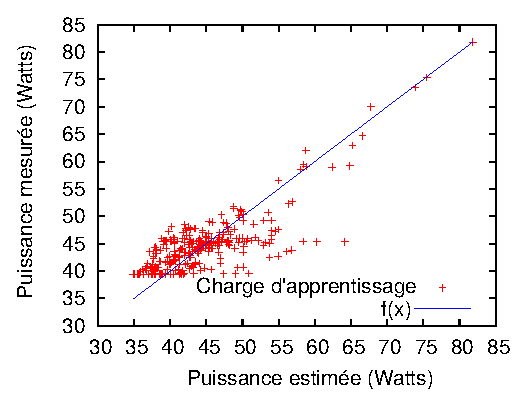
\includegraphics[width=0.5\textwidth]{chapitre4/chap4Fig/tpch-reg-poly-concurrent.eps}
  \caption{La qualité de la régression polynomiale pour la phase d'apprentissage du modèle de coût énergétique en mode concurrent.}\label{fig:tpch-reg-concurrent}
\end{figure}

Les résultats de la phase d'apprentissage comparés aux valeurs ajustées du modèle polynomial sont illustrés par la \ref{fig:tpch-reg-concurrent}. Comme nous pouvons voir sur la figure, la consommation d'énergie estimée et réelle rapprochent de près les lignes diagonales, indiquant ainsi la qualité de l'estimation que notre modèle peut générer. Il y a un certain écart entre l'estimation et l'énergie observée pour certains mixes de requêtes. Comme dans le cas du mode d'exécution isolé, une grande partie de ces erreurs est provoquée par l'optimiseur de requêtes, qui ne réussit pas à estimer les cardinalités de façon correcte lors de la phase de génération des plans d'exécution.

\subsubsection{Résultat avec des requêtes connues}
Pour évaluer notre modèle,  nous avons d'abord créé des charges de requêtes basées sur les modèles de requête TPC-H \textit{connus} d'une façon aléatoire. Pour chaque MPL, nous avons généré de nouveaux mixes à partir des 12 modèles, qui se traduit par 132 charges de requêtes.
%DONE idem que la previous todo 
Cependant, la génération aléatoire de mixes (échantillonnage) peut produire des mixes contenant les mêmes requêtes. Ainsi, cette technique ne couvre pas bien l'espace de mixes de requêtes possibles. Par conséquent, nous avons utilisé la méthode d'échantillonnage par hypercube latin (\gls{LHS}) \cite{Ahmad11}.
LHS crée un hypercube avec la même dimensionnalité que le nombre de modèles de requête \textit{T}. Chaque dimension est divisée en \textit{n} classes égales. La classe \textit{i} représente le nombre d'instances possibles du modèle de requête \textit{i}. LHS sélectionne alors \textit{n} mixes de l'espace de telle sorte que chaque classe de chaque modèle de requête apparaît dans exactement un mix. Intuitivement, LHS a une meilleure couverture de l'espace de mixes que la technique d'échantillonnage aléatoire.

\begin{figure}%[!ht]
  \centering
  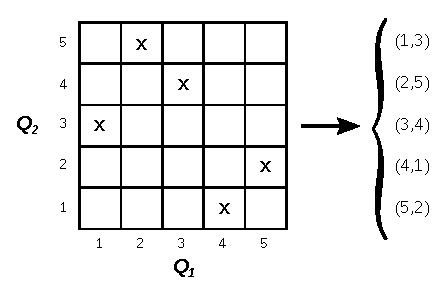
\includegraphics[width=0.5\textwidth]{chapitre4/chap4Fig/lhs.eps}
  \caption{Exemple d'échantillonnage par hypercube latin en 2-D.}\label{fig:lhs}
\end{figure}

La \ref{fig:lhs} montre un exemple où nous avons deux modèles de requête ($T = 2$), et nous devons sélectionner $n = 5$ mixes en utilisant LHS. Les deux axes $Q_1$ et $Q_2$ dans la figure désigne le nombre d'instances de requêtes de chaque type de requête dans un mix. La méthode d'échantillonnage par hypercube latin divise chacune de ces dimensions en 5 intervalles égaux. Les symboles << x >> désignent l'ensemble des mixes sélectionnés par la méthode LHS.

Nous avons testé la précision de la prédiction de notre modèle sur les mixes générés des modèles connus. La \ref{fig:tpch-test-all} montre les résultats des expérimentations.

\begin{figure}
 \centering
 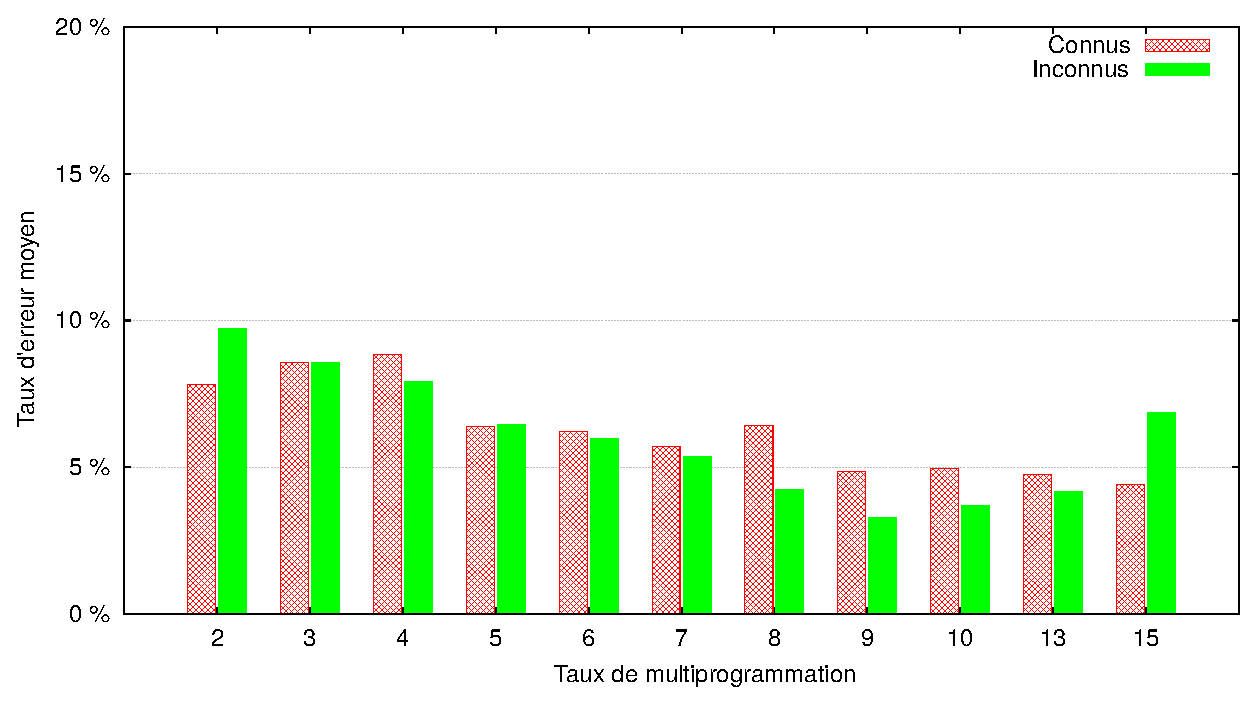
\includegraphics[scale=0.6]{chapitre4/chap4Fig/tpch-test-all.eps}
 \caption{Erreurs d'estimation d'énergie dans le benchmark TPC-H pour les modèles de requêtes connus et inconnus.}
 \label{fig:tpch-test-all}
\end{figure}

Comme illustré par la figure, l'erreur moyenne sur tous les est de 6,3\%  qui est considérée petite étant donné la variété de niveau de concurrence. En outre, l'erreur maximale est généralement inférieure à 9\%.

Notons en passant que nous pouvons voir que l'erreur est légèrement plus grande lorsque le MPL est petit (MPL = 2, 3 ou 4). Nous avons constaté que lorsque le MPL est élevé, la durée d'exécution des phases de pipeline est grande et notre modèle peut capturer leur consommation d'énergie. \`A l'inverse, lorsque le MPL est petit,  certaines phases de pipeline finissent leur exécution rapidement et notre modèle ne peut pas estimer leur consommation d'énergie avec précision. Ce problème est également observé dans certaines autres expérimentations.

\subsubsection{Résultat avec des requêtes inconnues}
Afin de tester notre modèle de coût contre de \textit{nouveaux} modèles de requêtes inconnues, nous avons créé des charges de requêtes basées sur le reste des requêtes du benchmark TPC-H qui ne sont pas utilisés dans la phase d'apprentissage, en utilisant la technique LHS. Plus précisément, pour chaque MPL nous avons généré 10 nouveaux mixes de requêtes, qui donnent lieu à 110 charges de requêtes.
%DONE idem, la je crois que cest vraiment charges de req :) -> ME: lol oui :)
 Les résultats sont présentés dans la \ref{fig:tpch-test-all}. On peut observer que les erreurs des prédictions du modèle de coût sont moins de 10\% pour les modèles de requêtes \textit{inconnus}, confirmant ainsi sa robustesse. %DONE a revoir ma reformulation

\subsubsection{Résultat avec un schéma complexe}
Pour vérifier la portabilité du modèle sur un nouveau schéma, nous avons choisi le schéma du benchmark TPC-DS. Nous nous sommes basés sur le même ensemble de 16 requêtes sélectionné dans le cas du mode d'exécution isolé. En utilisant la technique LHS, nous avons généré 16 mixes de requêtes pour chaque MPL, qui se traduit par 176 charges de requête. %DONE charges ou requetes :) je ne lache pas ;) -> ME: workload :)

La \ref{fig:tpcds-test-unknown} montre les résultats d'expérimentations. On peut observer que l'erreur des prédictions du modèle est inférieure à 10,5\%, ce qui montre que la modélisation de pipeline est un indicateur robuste pour la prédiction d'énergie dans le cas des données et des requêtes inconnues.

\begin{figure}
 \centering
 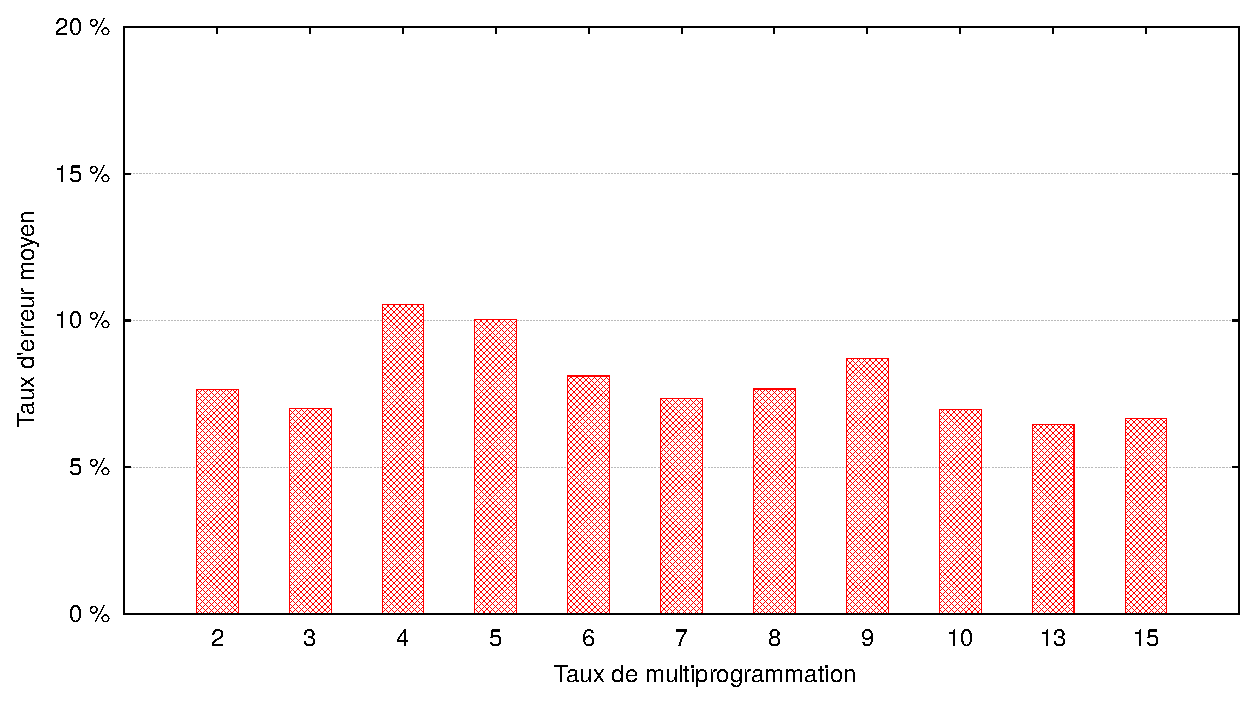
\includegraphics[scale=0.6]{chapitre4/chap4Fig/tpcds-test-unknown.eps}
 \caption{Erreurs d'estimation d'énergie dans les requêtes du benchmark TPC-DS en mode concurrent.}
 \label{fig:tpcds-test-unknown}
\end{figure}

\subsubsection{Résultat avec des charges de requêtes aléatoires}
Enfin, nous évaluons la précision de notre modèle pour prédire la consommation d'énergie pour tous les modèles de requête TPC-H de façon plus réaliste. Dans ces expérimentations et pour créer la charge de requêtes, nous passons par la liste de modèles de requêtes et nous ajoutons une instance de chaque modèle. En passant par la liste de modèles de nouveau d'une manière round-robin, nous continuons d'ajouter une instance de chaque modèle de requête à la charge jusqu'à ce que toutes les requêtes sont ajoutées. %TODO c'est moi qui s'est fatiguée ou je n'ai rien compris ?!! merci de revoir le paragraphe
En se basant sur les 22 requêtes de TPC-H, nous avons utilisé 4 instances pour chaque modèle de requêtes, ce qui résulte en une charge de 88 requêtes. Pour chaque MPL $M$, nous exécutons le premier mix de requête $M$, chaque fois qu'une requête se termine parmi les $M$ requêtes en cours d'exécution, une nouvelle requête à partir de la charge sera programmée à sa place sur la base de la politique d'ordonnancement First in, First out (FIFO). Cela nous donne une charge de requêtes d'une longue durée d'exécution qui prend en moyenne 2 heures pour terminer.

\begin{figure}
 \centering
 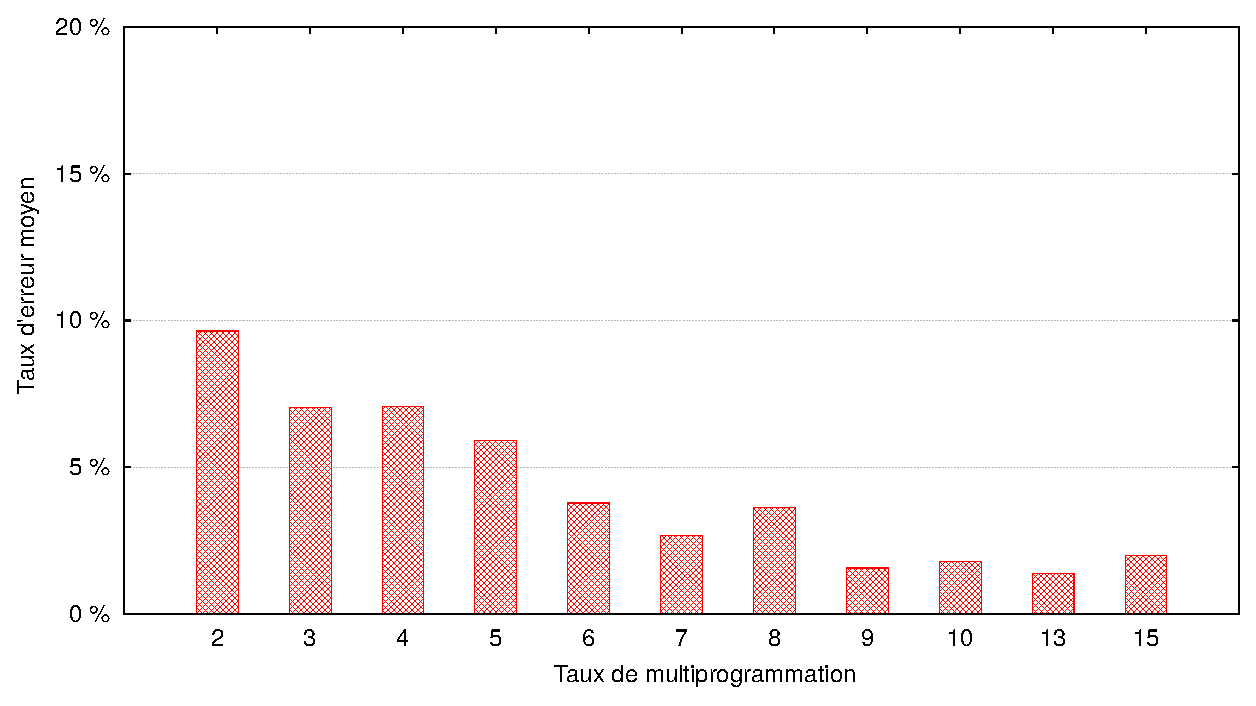
\includegraphics[scale=0.6]{chapitre4/chap4Fig/tpch-test-workload.eps}
 \caption{Erreurs d'estimation d'énergie dans le benchmark TPC-H pour tous les modèles de requêtes.}
 \label{fig:tpch-test-workload}
\end{figure}

Les résultats sont présentés dans la \ref{fig:tpch-test-workload}. Comme dans l'expérimentation précédente, les petits MPL  donnent des erreurs importantes par rapport aux grands MPL. Notre suggestion pour traiter ce scénario, est de modéliser l'énergie pour chaque groupe de MPL, par exemple, la création de modèle pour MPL $M1 \in \{2, \cdots, 5\}$, $M2 \in \{6, \cdots, 10\}$, $M3 \in \{11, \cdots, 15\}$ et ainsi de suite. Pour un futur travail, nous pouvons étendre notre framework avec une stratégie de regroupement similaire.
L'expérimentation montre que l'erreur d'estimation maximale est de 9,6\%. Ainsi, notre modèle peut faire face à des charges de requêtes réalistes.

\subsection{Bilan et discussion}
%TODO: add text
Les résultats expérimentaux ci-dessus indiquent clairement que notre modèle offre des résultats d'estimation d'énergie comparables à ceux donnés par les travaux connexes manipulant des modèles de requêtes connus exécutées en mode isolé \cite{Xu13, Kunjir12}. De plus, notre framework offre une amélioration significative par rapport aux techniques existantes, car il peut offrir une précision de prédiction similaire dans des scénarios plus complexes (à savoir des modèles de requêtes et des ensembles de données inconnus) et les requêtes exécutées en parallèle avec un taux de concurrence réaliste.

% Challenges and Limits

\section{Conclusion}
Dans nos jours, la consommation d'énergie des ordinateurs est devenue une préoccupation majeure pour l'industrie et la société. En conséquence, les chercheurs ont mis au point des techniques matérielles et logicielles pour assurer une efficacité énergétique.

Dans ce chapitre, nous proposons un modèle de coût basé sur les pipelines pour estimer la consommation d'énergie lors de l'exécution d'une requête SQL et un ensemble de requêtes exécutées simultanément.
Nous avons aussi indiqué comment la modélisation de pipeline pourrait être un indicateur robuste pour la prédiction d'énergie.
Le modèle de coût est construit sur la base des résultats empiriques obtenus à partir d'une charge de requêtes d'apprentissage qui a été soigneusement créée. Les paramètres matériels sont obtenues par un algorithme de régression polynomiale multiple.
En outre, nous avons effectué des tests sur notre modèle avec une BD réelle en exécutant un ensemble de requêtes, et avons comparé leurs coûts énergétiques avec ceux prédits par le modèle. Nos résultats montrent que le modèle, qui utilise uniquement des coûts de l'optimiseur en entrées, peut prédire l'énergie avec une petite erreur.
